
\section{Introduction}

As the development of technology of science and real life, the "big data" challenge becomes ubiquitous. Classical methods, such as Markov Chain Monte Carlo (MCMC), are normally suitable and good at handling a batch of data forecasting and analyzing. However, for big data and instant updating data stream, more robust and efficient methods are required. 


Alternative approaches, such as Sequential Monte Carlo, for on-line updating and estimating are well studied in scientific literature and quite prevalent in academic research in the last decades. When it embraced with  state space model, which is a very popular class of time series models that have found numerous of applications in fields as diverse as statistics, ecology, econometrics, engineering and environmental sciences \cite{cappe2009inference} \cite{smcmip2011} \cite{elliott1995estimation} \cite{cargnoni1997bayesian}, it allows us to establish complex linear and nonlinear Bayesian estimations in time series patterns \cite{vieira2016online}. 


\subsection*{State Space Model}

State space models are models that rely on the concept of state variables. If we describe a system as an operator mapping from the space of inputs to the space of outputs, then we may need the entire input-output history of the system together with the planned input in order to compute the future output values \cite{hangos2006analysis}. In an alternative way, by using new information at time $t$ containing all the past information up to the current state and initial conditions to get the current output is possible, that is known as a sequential method. A genetic state space model consists of two sets of equations: state equation and output equation. The state equation describes the evolution of the true input and state variables sequentially as a function and passes the variable one after one, generally, with some noises. The output equation catches the input values and interprets it out by an algebraic equation. A general state space model has the form form
\begin{align}\label{statemodel1}
\mbox{State equation } x_t &= G_t(x_{t-1})+w_t,\\
\label{statemodel2}
\mbox{Output equation } y_t &=F_t(x_t)+\epsilon_t
\end{align}
with an initial state $x_0$, where $\epsilon_t$ and $w_t$ are noise terms. $x_t$ are true status variables and $y_t$ are output values. Many researchers have been interested in this model and its application because of its good property. It can be used to model univariate or multivariate time series, and can be applied to system that exhibits non-stationarity, structural changes, and irregular patterns \cite{petris2009dynamic}.

The most simple and important system is given by Gaussian linear state space models, also known by dynamic linear models (DLM), which defines a very general class of non-stationary time series models.  Firstly, the model is linear, which means $G_t$ and $F_t$ are linear processes and satisfying linearity property. Secondly, the it is specified by a normal prior distribution for the $p$-dimensional state vector at initial state $t=0$, 
\begin{align*}
x_0 \sim N_p(m_0,C_0)
\end{align*} 
and two independent zero mean normal distributed noises $\epsilon_t \sim N_p(0,V_t)$ and $w_t \sim N_p(0,W_t)$ \cite{petris2009dynamic}. The well known Kalman Filter is a particular algorithm that is used to solve state space models in the linear case. This was first derived by Kalman \cite{kalman1960new}.

%In a nonlinear state space model, the process $G_t$ and $F_t$ are no longer linear functions and the situation becomes more complicated. Here gives a simple nonlinear example of such a model, which has been used extensively in the literature for benchmarking numerical filtering techniques \cite{kitagawa1996monte} \cite{west1993mixture} \cite{gordon1993novel} assuming the sequence is Markovian.
%\begin{align*}
%x_t &= \frac{x_{t-1}}{2} +25\frac{x_{t-1}}{1+x_{t-1}^2}+8\cos(1.2t)+u_t\\
%y_t &= \frac{x_{t}^2}{20}+v_t,
%\end{align*}
%where $u_t \sim N(0,\sigma_u^2)$, $v_t \sim N(0,\sigma_v^2)$, $\sigma_u^2=10$ and $\sigma_t^2=1$ are considered fixed and known. The initial state $x_0\sim N(0,10)$. 
The assumption Markovian keeps the current state $x_t$ only depending on the previous one step $x_{t-1}$ and the observed $y_t$ depending on $x_t$. A state-space is shown in the diagram below:
\begin{align*}
\begin{array}{cccccccccc}\cdots &\to &x_{t-1}&\to &x_{t}&\to &x_{t+1}&\to &\cdots &{\text{truth}}\\ \cdots &&\downarrow &&\downarrow &&\downarrow &&\cdots &\\ \cdots&&y_{t-1}&&y_{t}&&y_{t+1}&&\cdots &{\text{observation}}\end{array}
\end{align*}

In applications, the process function $G_t$ and $F_t$ contain unknown parameters to be estimated \cite{de1988likelihood} and the goal is to estimate the true states on sequential observations $y_t, \cdots, y_t$. Then it becomes to estimate a joint density of $p(x_{1:t},\theta \mid y_{1:t})$, where $x_{1:t} = \{x_1, x_2, \cdots, x_t \}$ are the hidden states and $y_{1:t} = \{y_1, y_2, \cdots, y_t \}$ are the observed outcomes and $\theta$ is a set of unknown parameters. 


\subsection*{Contents}

In this chapter, I will give a brief review on existing methods for sequential state and parameter inference. In section \ref{sectionFiltering}, I'm introducing some concepts and popular algorithms on estimating states sequentially. These algorithms are the fundamental of advanced methods. In section \ref{sectionStateandPara}, we will have a look at on-line algorithms that can estimate both unknown parameters and states simultaneously. In section \ref{sectionFilterreviewSimulation}, finally I will analyze these methods numerically and compare them with a proposed algorithm \ref{algorithmslidingwindow} in section \ref{SectionHighDimensionalOU}  with simulated data. 




\section{Filtering Problem and Estimation}\label{sectionFiltering}


\subsection{Sequential Monte Carlo Method}

The use of Monte Carlo methods for filtering can be traced back to the pioneering contributions of  \cite{handschin1969monte} and  \cite{handschin1970monte}. These researchers tried to use an importance sampling paradigm to approximate the target distributions and. Later on, an importance sampling algorithms were implemented sequentially in the filtering context. This algorithm is called sequential importance sampling, often abbreviated SIS, and has been known since the early 1970s. Limited by the power of computers and  suffering from sample impoverishment or weight degeneracy, the SIS didn't develop very well until 1993. Gordon used this a technique based on sampling and importance sampling methods to find the best state estimation  \cite{gordon1993novel}. A particle filter algorithm was proposed to allow rejuvenation of the set of samples by duplicating the samples with high importance weights and, on the contrary, removing samples with low weights \cite{cappe2009inference}. Since then, sequential Monte Carlo (SMC) methods have been applied in many different fields including but not limited to computer vision, signal processing, control, econometrics, finance, robotics, and statistics \cite{smcmip2011}  \cite{ristic2004beyond}.

In the state space model, a generic particle filter estimates the posterior distribution of the hidden states using the observation measurement process. The filtering problem is to estimate sequentially the values of the hidden states $x_t$ given the values of the observation process $y_{1:t}$ at any time $t$. In another word, it is to find the value of $p(x_t  \mid  y_{1:t})$. The process is divided into two steps: prediction and updating. In the prediction step, the assumption of Markov Chain is the current status $x_t $ only depends on the previous one $x_{t-1}$. Then we can calculate the probability of $x_t$ by 
\begin{align*}
p(x_t \mid y_{1:t-1})=&\int p(x_t ,x_{k-1}\mid y_{1:t-1}) dx_{t-1}\\
=&\int p(x_t \mid x_{t-1},y_{1:t-1}) p(x_{t-1}\mid y_{1:t-1})dx_{t-1}\\
=&\int p(x_t \mid x_{t-1}) p(x_{t-1}\mid y_{1:t-1})dx_{t-1}.
\end{align*}
In the updating step, once $p(x_t \mid y_{1:t-1})$ is known, $p(x_t \mid y_{1:t})$ can be found by
\begin{align*}
p(x_t \mid y_{1:t})=&\frac{p(y_t \mid x_t ,y_{1:t-1})p(x_{t}\mid y_{1:t-1})}{p(y_t \mid  y_{1:t-1})} \\
=&\frac{p(y_t \mid x_t )p(x_{t}\mid y_{1:t-1})}{p(y_t \mid  y_{1:t-1})},
\end{align*}
where the normalization $p(y_t \mid  y_{1:t-1})=\int p(y_t \mid x_t )p(x_t \mid  y_{1:t-1}) dx_t $ \cite{arulampalam2002tutorial}.

Imagine that the state space is partitioned as many parts, in which the particles are filled according to some probability measure. The higher probability, the denser the particles are concentrated. Suppose the particles $x_k^{(1)}, \ldots, x_k^{(N)}$ at time $k$ are drawn from the target probability density function $p(x)$, then these particles are used to estimate the expectation and variance of $f(x)$ by
\begin{align*}
\E(f(x)) &= \int_a^bf(x)p(x)dx\\
\Var(f(x)) &= \E\left[ f(x)-\E(f(x)) \right]^2p(x)dx.
\end{align*}
Back to our target, the posterior distribution or density is empirically represented by a weighted sum of samples $x_k^{(1)}, \ldots, x_k^{(N)}$  
\begin{equation}\label{rawParticleFilter}
\hat{p}(x_k\mid y_{1:t})=\frac{1}{N}\sum_{i=1}^N\delta \left(x_k-x_k^{(i)}\right)\approx p(x_k\mid y_{1:t}),
\end{equation}
where $f(x)=\delta (x_k-x_k^{(i)})$ is Dirac delta function. Hence, a continuous variable is approximated by a discrete one with a random support. When $N$ is sufficiently large, $\hat{p}(x_k\mid y_{1:t})$ was treated by particle filter as the true posterior $p(x_k\mid y_{1:t})$. By this approximation, the filtering problem becomes to get the expectation of current status 
\begin{align*}
\E(f(x_k)) &\approx \int f(x_k)\hat{p}(x_k\mid y_{1:t})dx_k \\
 & =\frac{1}{N} \sum_{i=1}^N\int f(x_k) \delta (x_k-x_k^{(i)}) dx_k\\
 & = \frac{1}{N}\sum_{i=1}^Nf\left(x_k^{(i)}\right).
\end{align*}
The expectation is the mean of the status of all particles $x_k^{(1)}, \ldots, x_k^{(N)}$.  

However, the posterior distribution is unknown and impossible to sample from the true posterior. To solve this issue, some sampling methods are introduced in the following sections.


\subsection{Importance sampling}

It is common to sample from an easy-to-implement distribution, the so-called proposal distribution $q(x\mid y)$, hence
\begin{align*}
\E\left(f(x)\right) &= \int f(x_t )\frac{p(x_t \mid y_{1:t})}{q(x_t \mid y_{1:t})} q(x_t \mid y_{1:t})dx_x\\
&= \int f(x_t )\frac{p(x_t )p(y_{1:t}\mid x_t )}{p(y_{1:t})q(x_t \mid y_{1:t})} q(x_t \mid y_{1:t})dx_x\\
&= \int f(x_t )\frac{W_t (x_t )}{p(y_{1:t})} q(x_t \mid y_{1:t})dx_x,
\end{align*}
where $W_t (x_t )=\frac{p(x_t )p(y_{1:t}\mid x_t )}{q(x_t \mid y_{1:t})} \propto \frac{p(x_t \mid y_{1:t})}{q(x_t \mid y_{1:t})}$. Because $p(y_{1:t})=\int p(y_{1:t}\mid x_t )p(x_t )dx_t $, so the above equation can be rewritten as
\begin{align*}
\E(f(x)) &= \frac{1}{p(y_{1:t})}\int f(x_t )W_t (x_t )q(x_t \mid y_{1:t})dx_t \\
&= \frac{ \int f(x_t )W_t (x_t )q(x_t \mid y_{1:t})dx_t  }{\int p(y_{1:t}\mid x_t )p(x_t )dx_t } \\
&= \frac{ \int f(x_t )W_t (x_t )q(x_t \mid y_{1:t})dx_t  }{\int W_t (x_t )q(x_t \mid y_{1:t})dx_t } \\
&= \frac{\E_{q(x_t \mid y_{1:t})}[W_t (x_t )f(x_t )]}{\E_{q(x_t \mid y_{1:t})}[W_t (x_t )]}.
\end{align*}
To solve the above equation, we can use Monte Carlo method by drawing samples $\{x_t^{(i)}\}$ from $q(x_t \mid y_{1:t})$ and get their expectation, which is  approximated by 
\begin{align}\label{PFexpectation}
\begin{split}
\E\left(f(x_t )\right) &\approx \frac{\frac{1}{N} \sum_{i=1}^{N} W_t\left(x_t^{(i)}\right)f\left(x_t^{(i)}\right)} {\frac{1}{N} \sum_{i=1}^{N} W_t\left(x_t^{(i)}\right)}\\
&= \sum_{i=1}^{N} \tilde{W}_t\left(x_t^{(i)}\right)f\left(x_t^{(i)}\right),
\end{split}
\end{align}
where $\tilde{W}_t\left(x_t^{(i)}\right) = \frac{ W_t\left(x_t^{(i)}\right)}{\sum_{i=1}^NW_t\left(x_t^{(i)}\right)}$ is factorized weight. Each particles has its own weighted value, so the expectation is a weighted mean. However, the drawback of this method is that the computation is quite expensive. A smarter way is to update $W_t^{(i)}$ recursively. Suppose the proposal distribution 
\begin{align*}
q(x_{0:t}\mid y_{1:t}) = q(x_{0:t-1}\mid y_{1:t-1}) q(x_t \mid  x_{0:t-1},y_{1:t}),
\end{align*}
then the recursive form of the posterior distribution is 
\begin{align*}
p(x_{0:t}\mid y_{1:t}) &= \frac{p(y_t \mid x_{0:t},y_{1:t-1})p(x_{0:t}\mid y_{1:t-1})}{p(y_t \mid y_{1:t-1})}\\
&= \frac{p(y_t \mid x_{0:t},y_{1:t-1}) p(x_t \mid x_{0:t-1},y_{1:t-1}) p(x_{0:t-1}\mid y_{1:t-1} ) }{p(y_t \mid y_{1:t-1})}\\
&= \frac{p(y_t \mid x_t ) p(x_t \mid x_{t-1}) p(x_{0:t-1}\mid y_{1:t-1} ) }{p(y_t \mid y_{1:t-1})}\\
&\propto p(y_t \mid x_t ) p(x_t \mid x_{t-1}) p(x_{0:t-1}\mid y_{1:t-1} ),
\end{align*}
the recursive form of the weights are
\begin{align*}
W_t^{(i)} &\propto \frac{p(x_{0:t}^{(i)}\mid y_{1:t})}{q(x_{0:t}^{(i)}\mid y_{1:t})}\\
&= \frac{ p(y_{1:t}\mid x_{0:t}^{(i)}) p(x_{t}^{(i)}\mid x_{t-1}^{(i)})  p(x_{0:t-1}^{(i)}\mid y_{1:t-1})}   { q(x_{t}^{(i)}\mid x_{0:t-1}^{(i)},y_{t})  q(x_{0:t-1}^{(i)}\mid y_{1:t-1}) } \\
&= W_{t-1}^{(i)} \frac{ p(y_{1:t}\mid x_{0:t}^{(i)}) p(x_{t}^{(i)}\mid x_{t-1}^{(i)}) }   {q(x_{t}^{(i)}\mid x_{0:t-1}^{(i)},y_{t})}.
\end{align*}

\subsection{Sequential Importance Sampling and Resampling}
 
In practice, we are interested in the current filtered estimate $p(x_t \mid y_{1:t})$ instead of $p(x_{0:t}\mid y_{1:t})$. Provided 
\begin{align*}
q(x_t \mid  x_{0:t-1},y_{1:t})=q(x_t \mid  x_{t-1},y_t ),
\end{align*}
the importance weights $W_t^{(i)}$ can be updated recursively via 
\begin{align*}
W_t^{(i)} &\propto W_{t-1}^{(i)} \frac{ p(y_t \mid x_t^{(i)}) p(x_{t}^{(i)}\mid x_{t-1}^{(i)}) }   {q(x_{t}^{(i)}\mid x_{t-1}^{(i)},y_{t})}.
\end{align*}

The problem of SIS filter is that the distribution of importance weights becomes more and more skewed as time increases. Hence, after some iterations, only very few particles have non-zero importance weights. This phenomenon is called \textit{weight degeneracy} or \textit{sample impoverishment} \cite{smcmip2011}.

The effective sample size $\textit{N}_{\textit{\tiny eff}}$ is suggested to monitor how bad the degeneration is, which is
\begin{align*}
\textit{N}_{\textit{\tiny eff}}=\frac{N}{1+\Var(w_t^{*(i)})},
\end{align*}
where $w_t^{*(i)}=\frac{p(x_t^{(i)}\mid y_{1:t})}{q(x_t^{(i)}\mid x_{t-1}^{(i)},y_{1:t})}$. The more different between the biggest weight and smallest weight, the worse the degeneration is. In practice, the effective sample size is approximated by
\begin{align*}
\hat{N}_{\textit{\tiny eff}}\approx \frac{1}{\sum_{i=1}^{N}\left(w_t^{(i)}\right)^2}.
\end{align*}
If the value of $\textit{N}_{\textit{\tiny eff}}$ is less than some threshold, some procedure should be used to avoid a worse degeneration. There are two ways one can do: choose an appropriate probability density function for importance sampling, or use resampling after SIS. 

The idea of resampling is keeping the same size of particles, replacing the low weights particles with new ones. As discussed before, 
\begin{align*}
p(x_t \mid y_{1:t})=\sum_{i=1}^Nw_t^{(i)} \delta \left(x_t -x_t^{(i)}\right).
\end{align*}
After resampling, it becomes
\begin{align*}
\tilde{p}(x_t \mid y_{1:t})=\sum_{j=1}^N\frac{1}{N} \delta \left(x_t -x_t^{(j)}\right)= \sum_{i=1}^N\frac{n_i}{N} \delta \left(x_t -x_t^{(i)}\right),
\end{align*}
where $n_i$ represents how many times the new particles $x_t^{(j)}$ were duplicated from$x_t^{(i)}$. 

Then the process of SIS particle filter with resampling is:
%\begin{itemize}
%\item Initial particles when $t=0$. For $i=1, \ldots, N$, draw samples $\{x_0^{(i)}\}$ from $p(x_0)$.
%\item For $t=1,2,\ldots$, run the process recursively
%\begin{itemize}
%\item Importance sampling: draw sample $\{\tilde{x}_t^{(i)}\}_{i=1}^N$ from $q(x_t \mid y_{1:t})$, calculate their weights $\tilde{w}_t^{(i)}$ and normalize them.
%\item Resampling: Resample $\{\tilde{x}_t^{(i)}, \tilde{w}_t^{(i)}\}$ and get a new set $\{x_t^{(i)},\frac{1}{N}\}$.
%\item Output the status at time $t$: $\hat{x}_t =\sum_{i=1}^{N}\tilde{x}_t^{(i)}\tilde{w}_t^{(i)}$.
%\end{itemize}
%\end{itemize}
\begin{algorithm}[h]
\SetAlgoLined 
%\KwResutt{Write here the resutt }
Initialization: Initial particles when $t=0$. For $i=1, \ldots, N$, draw samples $\{x_0^{(i)}\}$ from $p(x_0)$.\\
\For{$t=1,2,\ldots, n$} {Importance sampling: draw sample $\{\tilde{x}_t^{(i)}\}_{i=1}^N$ from $q(x_t \mid y_{1:t})$, calculate their weights $\tilde{w}_t^{(i)}$ and normalize them. \\
Resampling: Resample $\{\tilde{x}_t^{(i)}, \tilde{w}_t^{(i)}\}$ and get a new set $\{x_t^{(i)},\frac{1}{N}\}$.\\
Output the status at time $t$: $\hat{x}_t =\sum_{i=1}^{N}\tilde{x}_t^{(i)}\tilde{w}_t^{(i)}$.}
 \caption{Sampling and Importance Sampling.}\label{algorithmSIS}
\end{algorithm}


In SIR, if we choose
\begin{align*}
q(x_t^{(i)}\mid x_{t-1}^{(i)},y_t ) = p(x_t^{(i)}\mid x_{t-1}^{(i)}),
\end{align*}
the weights become
\begin{align*}
w_t^{(i)}&\propto w_{t-1}^{(i)}\frac{ p(y_t \mid x_{t}^{(i)}) p(x_t^{(i)}\mid x_{t-1}^{(i)}) }{q(x_t^{(i)}\mid x_{t-1}^{(i)},y_t ) }\\
&\propto w_{t-1}^{(i)}p(y_t \mid x_{t}^{(i)}).
\end{align*}
Because $w_{t-1}^{(i)}=\frac{1}{N}$, thus we have $w_t^{(i)} \propto p(y_t \mid x_{t}^{(i)})$ and
\begin{align*}
w=\frac{1}{\sqrt{2\pi\Sigma}}\exp\left(-\frac{1}{2} (y_{\mbox{\tiny true}}-y)\Sigma^{-1}(y_{\mbox{\tiny true}}-y)\right).
\end{align*}

However, SMC methods are suffering some drawbacks. At any time point $k (k<t)$, if $t-k$ is too large, the approximation to marginal $p(x_k\mid y_{1:t})$ is likely to be rather poor as the successive resampling steps deplete the number of distinct particle co-ordinates $x_k$ \cite{andrieu2010particle}, which is also the difficulty of approximating $p(\theta,x_{1:t}\mid y_{1:t})$ with SMC algorithms 
\cite{andrieu1999sequential} \cite{fearnhead2002markov} \cite{storvik2002particle}. 




\subsection{Auxiliary Particle Filter}

The auxiliary particle filter (APF) was first introduced in \cite{pitt1999filtering} as an extension of SIR to perform inference in state space model. The author uses the idea of stratification into particle filter to solve particle degeneracy by pre-selecting particles before propagation. 

At each step, the algorithm draws a sample of the particle index $i$, which will be propagated from $t-1$ into the $t$, on the mixture in (\ref{PFexpectation}). These indexes are auxiliary variables only used as an intermediary step, hence the name of the algorithm \cite{pitt1999filtering}. Thus, the task becomes to sample from the joint density $p(x_t,i\mid y_{1:t})$. Define 
\begin{equation}
p(x_t,i\mid y_{1:t})\propto p(y_t\mid x_t)p(x_t\mid x_{t-1}^{(i)})w_{t-1}^{(i)}, 
\end{equation}
and define $\mu_t^{(i)}$ as some characterization of $x_t\mid x_{t-1}$, which suggested by the author could be mean, mode, a sample and so on, then the joint density can be approximated by  
\begin{equation}
\pi(x_t,i\mid y_{1:t})\propto p(y_t\mid \mu_t^{(i)})p(x_t\mid x_{t-1}^{(i)})w_{t-1}^{(i)}, 
\end{equation}
with weights
\begin{equation*}
w_t^{(i)}\propto \frac{ p(y_t\mid x_t^{(i)})  }{  p(y_t\mid\mu_t^{k(i)})   }.
\end{equation*}
This auxiliary variable based SIR requires only the ability to propagate and evaluate the likelihood, just as the original SIR suggestion of \cite{gordon1993novel}.  

The main idea behind the APF, that is modifying the original sequence of target distributions to guide particles in promising regions, can be extended outside the filtering framework \cite{JOHANSEN20081498}. It is also recommended in the literature \cite{liu2008monte} that the particles can be re-sampled not according to the normalized weights $w_t^{\mbox{\tiny SISR}}(x_{1:t})=\frac{p(x_{1:t})}{ p(x_{1:t-1}q(x_t\mid x_{1:t-1})  }$  but according to a generic score function $w_t(x_{1:t})>0$ at time t
\begin{equation*}
w_t(x_{1:t}) = g(w_t^{\mbox{\tiny SISR}}(x_{1:t})),
\end{equation*}
where $g: \mathbb{R}^+\rightarrow \mathbb{R}^+$ is a monotonously increasing function, such as $g(x)=x^\alpha$, where $0<\alpha\leq 1$. 



\subsection{Sequential Particle Filter}


SMC method is effective for exploring the sequence of posteriors distribution  $\pi(x_t\mid\theta) = p(x_t\mid y_{1:t},\theta)$, where the static parameters are
treated as known. An inference about $\pi_{t-1}$ is used to draw an inference on $\pi_t$ by SIS and resampling. Its interest is focused on $x_t$ instead of the whole path $x_{0:t}$, that is the filtering problem. However, this algorithm evolves, weights and resamples a population of $N$ number of particles, $x_t^{(1)},\ldots,x_t^{(N)}$, so that at each time $t$ they are a properly weighted sample from $\pi(x_t \mid \theta)$. Additionally, it is not practicable on huge datasets, because of numerous iterations in sampling process. 

As a complementary solution, sequential particle filter method was proposed by Nicolas \cite{chopin2002sequential} as the first part of his Ph.D. thesis. Instead, sequential particle filter is using preliminary explorations of partial distribution $\pi(\theta\mid y_{1:k})$ $(k<t)$. The concept is: an inference of $\pi(\theta)$ is drawn from the first $k$ observations, let's name it "learning phase", and it is then updated through importance sampling to incorporate the following $l$ observations, name it "updating phase", \cite{chopin2002sequential}.  This method is named as iterated batch importance sampling (IBIS) algorithm, which is used for the recursive exploration of the sequence of parameter posterior distributions $\pi(\theta)$. It updates a population of $N$ particles for $\theta$, $\theta^{(1)}, \ldots, \theta^{(N)}$, so that at each time $t$ they are a properly weighted sample from $\pi(\theta)$. The algorithm includes occasional MCMC steps for rejuvenating the current population of particles of $\theta$  to prevent the number of distinct from decreasing over time. 

In a batch mode, we are assuming the parameter $\theta$ is static. When the first $k$ observations become available, we can find the posterior distribution is $\pi(\theta\mid y_{1:k})$. After that, a few $l (l<\infty)$ observations come into data stream, the posterior becomes $\pi(\theta\mid y_{1:k+l})$ and it is likely to be similar with $\pi(\theta\mid y_{1:k})$.  Hence, a proper reweighting particles by the incremental weight is 
\begin{align*}
w_{k,l}(\theta) &\propto \frac{\pi(\theta\mid y_{1:k+l}) }{\pi(\theta\mid y_{1:k}} \\
&\propto \frac{p(y_{1:k+l}\mid \theta) }{p(y_{1:k}\mid\theta)} \\
&=p(y_{k+1:k+l}\mid y_{1:k},\theta). 
\end{align*}

Sequentially, the iterated batch importance sampling algorithm is in the following 
%\begin{itemize}
%\item{Step 1.} Initialization. General particles of $\theta_i$ and $w_i$, $i=1,\ldots,N$. 
%\item{Step 2.} Re-weighting. Update the weights by $w_i^*=w_i \times w_{k,l}$, where $w_{k,l}(\theta_i)\propto p(y_{k+1:k+l}\mid y_{1:k},\theta_i)$, $i=1,\ldots,N$. 
%\item{Step 3.} Resampling. Normalize $\theta_i$ and $w^*_i$ to $\theta_i^*$ and $\frac{1}{N}$ according to $p(\theta_i^*=\theta_i)=\frac{w_i^*}{\sum w_i^*}$,  $i=1,\ldots,N$. 
%\item{Step 4.} Propagating. Draw $\theta_i^m$ from $K_{k+l}(\theta_i^*)$, where $K_{k+l}$ is a predefined transition kernel function with stationary distribution $\pi_{k+l}$.
%\item{Step 5.} Set $(\theta_i^m,\frac{1}{N})$ to $(\theta_i,w_i)$, $k+l$ to $k$ and return to reweighting step. 
%\end{itemize}
%The algorithm stops when $k=t$, that is when the particle system targets the distribution of interest $\pi(\theta\mid y_{1:t})$. 
\begin{algorithm}[h]
\SetAlgoLined 
%\KwResutt{Write here the resutt }
Initialization:  General particles of $\theta_i$ and $w_i$, $i=1,\ldots,N$.\\
\While{$k<t$} {Re-weighting. Update the weights by $w_i^*=w_i \times w_{k,l}$, where $w_{k,l}(\theta_i)\propto p(y_{k+1:k+l}\mid y_{1:k},\theta_i)$, $i=1,\ldots,N$. \\
Resampling. Normalize $\theta_i$ and $w^*_i$ to $\theta_i^*$ and $\frac{1}{N}$ according to $p(\theta_i^*=\theta_i)=\frac{w_i^*}{\sum w_i^*}$,  $i=1,\ldots,N$. \\
Propagating. Draw $\theta_i^m$ from $K_{k+l}(\theta_i^*)$, where $K_{k+l}$ is a predefined transition kernel function with stationary distribution $\pi_{k+l}$.\\
Set $(\theta_i^m,\frac{1}{N})$ to $(\theta_i,w_i)$, $k+l$ to $k$.}
 \caption{Sequential Particle Filter.}\label{algorithmSequentialPF}
\end{algorithm}
The algorithm stops when $k=t$, that is when the particle system targets the distribution of interest $\pi(\theta\mid y_{1:t})$. 


\subsection{MCMC-Based Particle Algorithm}

Markov Chain Monte Carlo (MCMC) methods are a set of powerful stochastic algorithms that allow us to solve most of these Bayesian computational problems when the data are available in batches \cite{tierney1994markov}. However, as data set becomes larger and larger, it requires numerous computing in the process. Sequential Monte Carlo approaches have become a powerful methodology to cope with large data set recursively. However, it is inefficient when applied to high dimensional problems \cite{septier2009mcmc}. A nature extension is whether there exists a sequential MCMC method to diversify the degenerate particle population thus improving the empirical approximation for multi-target tracking or high dimensional space. Luckily, sequential approaches using MCMC were proposed in \cite{berzuini1997dynamic}, in which the author combine MCMC with importance resampling to sequentially update the posterior distribution. 
Other discussions, such as \cite{khan2005mcmc}, \cite{golightly2006bayesian} and \cite{pang2008models}, are using either resampling nor importance sampling. 

As we discussed before, the a filtering problem is to find the posterior distribution recursively, like 
\begin{equation}
p(x_t\mid y_{1:t}) \propto \int p(y_t\mid x_t)p(x_t\mid x_{t-1})p(x_{t-1}\mid y_{1:t-1})dx_{t-1}. 
\end{equation} 
In particle filter, the posterior is approximated by particles $x_t^{(1)},\ldots,x_t^{(N)}$ in equation (\ref{rawParticleFilter}). A MCMC procedure is designed using (\ref{rawParticleFilter}) as the target distribution with a proposal distribution of $q(x_t\mid x_t^{(i)})$. Therefore, like MCMC, the desired approximation $\hat{p}(x_t\mid y_{1:t})$ is obtained by storing every accepted samples after the initial burn-in iterations \cite{septier2009mcmc}. The drawback is excessive computation occurs as the number of particles increases at each iteration. 

To avoid this issue, a MCMC-based particle algorithm in \cite{pang2008models} considers the joint posterior distribution of $x_t$ and $x_{t-1}$:
\begin{equation}
p(x_t,x_{t-1}\mid y_{1:t})\propto p(y_t\mid x_t)p(x_t\mid x_{t-1})p(x_{t-1}\mid y_{1:t-1}),
\end{equation}
which becomes the new target distribution. At the $i$th sampling iteration, the joint $x_k$ and $x_{k-1}$ was proposed in a Metropolis-Hastings sampling step. After that, a refinement Metropolis-within-Gibbs step update $x_k$ and $x_{k-1}$ individually. Hence, the algorithm is summarized in algorithm \ref{algorithmMCMCParticle}:
%\begin{itemize}
%\item Initialize particles $x_0^{(1)},\ldots,x_0^{(N)}$.
%\item Propose $\{x_k^*,x_{k-1}^*\}\sim q_1(x_k,x_{k-1}\mid x_{k}^{(i-1)},x_{k-1}^{(i-1)})$.
%\item Accept $\{x_k^*,x_{k-1}^*\}$ with probability $\alpha_1=\min\lbrace 1, \frac{ p(x_k^*,x_{k-1}^*\mid y_{1:t} )  }{ p(x_k^{(i-1)},x_{k-1}^{(i-1)}\mid y_{1:t} )  }  \frac{ q_1(x_k^{(i-1)},x_{k-1}^{(i-1)}\mid x_k^*,x_{k-1}^*)  }{ q_1(x_k^*,x_{k-1}^* \mid x_k^{(i-1)},x_{k-1}^{(i-1)})  }   \rbrace$
%\item Propose $x_{k-1}^*\sim q_2(x_{k-1}\mid  x_k^{(i)},x_{k-1}^{(i)}  )$
%\item Accept $x_{k-1}^*$ with probability $\alpha_2 = \min \lbrace 1, \frac{ p(x_{k-1}^*\mid x_k^{(i)},y_{1:t}) }{  p(x_{k-1}^{(i)}\mid x_{k}^{(i)},y_{1:t})  }  \frac{ q_2(x_{k-1}^{(i)} \mid x_{k-1}^*, x_k^{(i)} ) }{ q_2(x_{k-1}^*\mid x_{k}^{(i)},x_{k-1}^{(i)})    } \rbrace$
%\item Propose $x_k^* \sim q_3(x_k\mid x_k^{(i)}, x_{k-1}^{(i)})$
%\item Accept $x_k^*$ with probability $\alpha_3 =\min \lbrace 1,
%\frac{ p(x_{k}^*\mid x_{k-1}^{(i)},y_{1:t}) }{  p(x_{k}^{(i)}\mid x_{k-1}^{(i)},y_{1:t})  }  \frac{ q_3(x_{k}^{(i)} \mid x_{k}^*, x_{k-1}^{(i)} ) }{ q_3(x_{k}^*\mid x_{k}^{(i)},x_{k-1}^{(i)}) }  \rbrace  $
%\item After burn-in points, keep $x_k^{(j)}$ as new particles for approximating.
%\item Move to next particle $i+1$
%\item Move to next state $k+1$
%\end{itemize}
\begin{algorithm}[h]
\SetAlgoLined 
%\KwResutt{Write here the resutt }
Initialization: Initialize particles $x_0^{(j)}, j =1, \ldots,N$. \\
\For{$k = 1,\ldots,t$}{
\For{$i = 1,\ldots,M$}{
Propose $\{x_k^*,x_{k-1}^*\}\sim q_1(x_k,x_{k-1}\mid x_{k}^{(i-1)},x_{k-1}^{(i-1)})$. \\
Accept $\{x_k^*,x_{k-1}^*\}$ with probability $\alpha_1=\min\lbrace 1, \frac{ p(x_k^*,x_{k-1}^*\mid y_{1:t} )  }{ p(x_k^{(i-1)},x_{k-1}^{(i-1)}\mid y_{1:t} )  }  \frac{ q_1(x_k^{(i-1)},x_{k-1}^{(i-1)}\mid x_k^*,x_{k-1}^*)  }{ q_1(x_k^*,x_{k-1}^* \mid x_k^{(i-1)},x_{k-1}^{(i-1)})  }   \rbrace$\\
Propose $x_{k-1}^*\sim q_2(x_{k-1}\mid  x_k^{(i)},x_{k-1}^{(i)}  )$ \\
Accept $x_{k-1}^{(i)} = x_{k-1}^*$ with probability $\alpha_2 = \min \lbrace 1, \frac{ p(x_{k-1}^*\mid x_k^{(i)},y_{1:t}) }{  p(x_{k-1}^{(i)}\mid x_{k}^{(i)},y_{1:t})  }  \frac{ q_2(x_{k-1}^{(i)} \mid x_{k-1}^*, x_k^{(i)} ) }{ q_2(x_{k-1}^*\mid x_{k}^{(i)},x_{k-1}^{(i)})    } \rbrace$. \\
Propose $x_k^* \sim q_3(x_k\mid x_k^{(i)}, x_{k-1}^{(i)})$. \\
Accept $x_{k}^{(i)} =x_k^*$ with probability $\alpha_3 =\min \lbrace 1,
\frac{ p(x_{k}^*\mid x_{k-1}^{(i)},y_{1:t}) }{  p(x_{k}^{(i)}\mid x_{k-1}^{(i)},y_{1:t})  }  \frac{ q_3(x_{k}^{(i)} \mid x_{k}^*, x_{k-1}^{(i)} ) }{ q_3(x_{k}^*\mid x_{k}^{(i)},x_{k-1}^{(i)}) }  \rbrace$.\\
After burn-in points, keep $x_k^{(j)}= x_k^{(i)}$ as new particles for approximating $p(x_k\mid y_{1:k})$.\\
}
}
 \caption{MCMC-Based Particle Algorithm.}\label{algorithmMCMCParticle}
\end{algorithm}

In \cite{septier2009multiple}, the authors discussed some attractive features of genetic algorithms and simulated annealing into the framework of MCMC based particle scheme. One may refer to the paper for details. 




\section{On-line State and Parameters Estimation}\label{sectionStateandPara}

The state transition density and the conditional likelihood function depend not only upon the dynamic state $x_t$, but also on a static parameter vector $\theta$, which will be stressed by use of the notations $f(x_t \mid x_{t-1},\theta)$ and $g(y_t\mid x_t,\theta)$. Putting the algorithms on-line means to update the parameters and states instantly as new observations coming into the data stream. For Bayesian dynamic models, however, the most natural option consists in treating the unknown parameter $\theta$, using the state space representation, as a component of the state which has no dynamic evolution, also referred to as a static parameter \cite{cappe2007overview}. The standard SMC is deficiency for on-line parameter estimation. As a result of the successive resampling steps, after a certain time $t$, the approximation $\hat{p}(\theta\mid y_{1:t})$ will only contain a single unique value for $\theta$. In other words, SMC approximation of the marginalized parameter posterior distribution is represented by a single Dirac delta function. It also causes error accumulation in successive Monte Carlo (MC) steps grows exponentially or polynomially in time \cite{kantas2009overview}. 

Therefore, in this section, we are introducing some methods that will estimate combined state and parameter by either jointly estimating of state and parameter or by marginalizing the parameter using sufficient statistics. 





\subsection{Artificial Dynamic Noise}\label{ArtificialNoise}

Some methods are trying to solve the posterior distribution $p(\theta \mid y_{1:t})$ by 
\begin{equation}
p(\theta \mid y_{1:t}) \propto p(y_{1:t} \mid \theta ) p(\theta )
\end{equation}
through maximize the likelihood function without introducing any bias or controlling the bias in states propagation. A pragmatic approach to reduce parameter sample degeneracy and error accumulation in successive MC approximations is to adding an artificial dynamic equation on $\theta$ \cite{higuchi2001self} \cite{kitagawa1998self}, which gives
\begin{align*}
\theta_{n+1} = \theta_n+\varepsilon_{n+1}.
\end{align*}
The artificial noise $varepsilon_{t+1}\sim N(0,W_{t+1})$ is specified by covariance matrix $W_{t+1}$. With this noise, SMC can now be applied to approximate $p(x_{1:t},\theta\mid y_{1:t})$. A related kernel density estimation method proposes a kernel density estimate of the target \cite{liu2001combined} \begin{align*}
\hat{p}(\theta\mid y_{1:t}) = \frac{1}{N}\sum M(\theta-\theta_n^{(i)}). 
\end{align*} 
At time $t+1$, the samples obtain a new set of particles. 


\subsection{Practical Filtering}

A fixed-lag approach to filtering and sequential parameter learning was proposed in \cite{polson2008practical}. Its key idea is to express the the filtering distribution as a mixture of lag-smoothing distributions and to implement it sequentially. 

With a fixed-lag $l$, the state filtering and parameter learning require the sequence of the joint distribution $p(x_t,\theta\mid y_{1:t})$, which implies the desired filtering distribution $p(x_t\mid y_{1:t})$ being marginalized as 
\begin{equation*}
p(x_t\mid y_{1:t}) = \int p(x_{t-l+1:t}\mid y_{1:t}) dx_{t-l+1:t-1},
\end{equation*}
and the parameter posterior distribution $p(\theta\mid y_{1:t})$. Arguing that the approximation that draws from $p(x_{0:t-l}\mid y_{1:t-1})$ are approximate draws from $p(x_{0:t-l}\mid y_{1:t})$, the state filtering with static parameter $\theta$ is 
\begin{align*}
p(x_{t-l+1:t},\theta\mid y_{1:t}) &=\int p(x_{t-l+1,t},\theta \mid x_{0:t-l},y_{1:t}) dp(x_{0:t-l}\mid y_{1:t}) \\
&\approx \int p(x_{t-l+1,t},\theta \mid x_{0:t-l},y_{1:t}) dp(x_{0:t-l}\mid y_{1:t-1}).
\end{align*}
Therefore, we can firstly draw some samples $x_{0:t-l}^{(i)}$ from $p(x_{0:t-l}\mid y_{1:t-1})$, which is approximately the same as $p(x_{0:t-l}\mid y_{1:t})$ and $i=1,\ldots,M$. Then, use these samples to estimate states and parameter by 
\begin{align*}
x_{t-l+1} &\sim p(x_{t-l+1}\mid x_{0:t-l}^{(i)},\theta,y_{t-l+1:t}),\\
\theta &\sim p(\theta \mid x_{0:t-l}^{(i)},x_{t-l+1},y_{t-l+1:t}),
\end{align*}
with two-step Gibbs sampler. The algorithm is summarized below:

%\begin{itemize}
%\item{Step 1.} Initialization. Set $\theta^{(i)}=\theta_0$ as initial values, $i=1,\ldots,N$. 
%\item{Step 2.} Burn in: For $k=1,\ldots,l$, initialize $\theta = \theta^{(i)}$. Generate $x_{0:k}\sim p(x_{0:k}\mid \theta,y_{1:k})$ and $\theta \sim p(\theta\mid x_{0:k},y_{1:k})$.
%\item{Step 3.} Achieve a set of $\left( x_{0:k}^{(i)},\theta^{(i)}\right)$.
%\item{Step 4.} Sequential updating: For $k=l+1,\ldots,t$: initialize $\theta = \theta^{(i)}$. Generate $x_{k-l+1:k}\sim p(x_{k-l+1:k}\mid x_{k-l}^{(i)},\theta,y_{k-l+1,k})$ and $\theta \sim p(\theta\mid x_{0:k-l}^{(i)},x_{k-l+1:k},y_{1:k})$. 
%\item{Step 5.} Achieve a set of $\left( x_{k-l+1}^{(i)},\theta^{(i)}\right)$ and leave $x_{0:k-l}^{(i)}$ unchanged. 
%\end{itemize}
\begin{algorithm}[h]
\SetAlgoLined 
%\KwResutt{Write here the resutt }
Initialization: Set $\theta^{(i)}=\theta_0$ as initial values, $i=1,\ldots,N$.  \\
Burn-In: \For{$k = 1,\ldots, l$}{
\For{$i=1,\ldots,N$}{Initialize $\theta = \theta^{(i)}$. \\
Generate $x_{0:k}\sim p(x_{0:k}\mid \theta,y_{1:k})$ and $\theta \sim p(\theta\mid x_{0:k},y_{1:k})$.\\
After a few iterations, achieve a set of $\{ \tilde{x}_{0:k}^{(i)},\theta^{(i)}\}$. 
}
}
Sequential Updating: \For{$k=l+1,\ldots,t$}{
\For{$i=1,\ldots,N$}{initialize $\theta = \theta^{(i)}$.\\
Generate $x_{k-l+1:k}\sim p(x_{k-l+1:k}\mid \tilde{x}_{k-l}^{(i)},\theta,y_{k-l+1,k})$ and $\theta \sim p(\theta\mid \tilde{x}_{0:k-l}^{(i)},x_{k-l+1:k},y_{1:k})$. \\
Achieve a set of $\{ \tilde{x}_{k-l+1}^{(i)},\theta^{(i)}\}$ and leave $\tilde{x}_{0:k-l}^{(i)}$ unchanged.
}
}
 \caption{Practical Filtering Algorithm.}\label{algorithmPraticalFilter}
\end{algorithm}

The speed and accuracy of this algorithm depends on the choice of sample size $M$ and the lag $l$, which is difficult, and there is a non-vanishing bias which is difficult to quantify \cite{polson2008practical} \cite{kantas2009overview}.




%A MCMC kernel with invariant density $p(x_{1:t},\theta\mid y_{1:t})$ is used in SMC algorithm. This method was firstly used in an on-line Bayesian parameter estimation, where the author in \cite{andrieu1999sequential} were using
%\begin{align*}
%K_n(x_{1:t}',\theta'\mid x_{1:t},\theta) = \delta_{x_{1:t}}(x_{1:t} ')p(\theta'\mid x_{1:t},y_{1:t}),
%\end{align*}
%where $p(y_{1:t}\mid\theta,x_{1:t})=p(\theta\mid s_t(x_{1:t},y_{1:t}))$ and $s_t(x_{1:t},y_{1:t})$ is a fixed-dimensional vector of sufficient statistics. MCMC can be used to maintain the diversity of the samples of $\theta$. Here the stationary distribution for the MCMC will be the full joint posterior distribution of states and parameters and apply MH or Gibbs sampling separately to $p(\theta \mid x_{1:t},y_{1:t})$ and $p(x_{1:t} \mid \theta,y_{1:t})$. However, this method is not feasible for large dataset. 



% % % % % % % % % % % % % % % % % % % % % % % % % % % %
% % % % % % % % % % % % % % % % % % % % % % % % % % % %



\subsection{Liu and West's Filter}

Particles degeneracy is inevitable in SMC. Method in section \ref{ArtificialNoise} reduce the degeneracy by adding artificial noise to the parameters, however, that will also lead to the variance of estimates. Liu and West in \cite{liu2001combined} used a kernel smoothing approximation combined with a neat shrinkage idea to kill over-dispersion. 

At time $t$, suppose we have particles $\{x_t^{(i)}\}$ and associated weights $\{w_t^{(i)}\}$, $i=1,\ldots,N$, Bayes' theorem tells us that approximation to the posterior distribution $p(x_{t+1}\mid y_{1:t+1})$ at time $t+1$ of the state is 
\begin{equation*}
p(x_{t+1} \mid y_{1:t+1}) \propto \sum_{i=1}^{N} w_t^{(i)} p(x_{t+1} \mid x_t^{(i)})p(y_{t+1}\mid x_{t+1}).
\end{equation*}
However, variance increases through over $t$ by the Gaussian mixture. In \cite{west1993mixture}, the author is a smooth kernel density 
\begin{equation}\label{LiuandWestDensity}
p(\theta\mid y_{1:t})\approx \sum_{i=1}^{N}w_t^{(i)} N(\theta\mid m_t^{(i)},h^2V_t)
\end{equation}
to against the sample dispersion. Because $N(\cdot\mid m,C)$ is a multivariate normal density with mean $m$ and covariance matrix $C$, so the above density (\ref{LiuandWestDensity}) is a mixture of $N(\theta\mid m_t^{(i)},h^2V_t)$ distribution weighted by the sample weights $w_t^{(i)}$. Without this shrinkage approach, the standard kernel locations would be $m_t^{(i)}=\theta_t^{(i)}$, by which there is an over dispersed kernel density, because of $(1=h^2)V_t$ is always large than $V_t$. $\theta_t$ indicates the samples are from the time $t$ posterior, not time-varying. 

To correct it, the idea of shrinkage kernel is 
\begin{equation}
m_t^{(i)}=\alpha \theta_t^{(i)} + (1-\alpha)\bar{\theta}_t,
\end{equation}
where $\alpha=\sqrt{1-h^2}$ and $h>0$ is the smoothing parameter and the covariance is $V_t=\sum_{i=1}^{N}\frac{ (\theta_t^{(i)}-\bar{\theta}_t )(\theta_t^{(i)}-\bar{\theta}_t  )^\top}{N}$. Consequently, the resulting normal mixture retains the mean $\bar{\theta}_t$ and now has the correct covariance $V_t$, hence the over dispersion is trivially corrected \cite{liu2001combined}. 

A general algorithm is summarized bellow: 
%\begin{itemize}
%\item{Step 1.} Identify the prior estimation of $(x_t,\theta)$ by $(\mu_{t+1}^{(i)},m_t^{(i)})$, where
%$\mu_{t+1}^{(i)}=\E (x_{t+1}\mid x_t^{(i)},\theta_t^{(i)})$, and $m_t^{(i)}=\alpha \theta_t^{(i)} + (1-\alpha)\bar{\theta}_t$.
%\item{Step 2.} Sample an auxiliary integer index $k$ from $\{1,\ldots,N\}$ with probability proportional to $g_{t+1}^{(i)}\propto w_t^{(i)}p(y_{t+1}\mid \mu_{t+1}^{(i)},m_t^{(i)})$.
%\item{Step 3.} Sample a new parameter vector $\theta_{t+1}^{(k)}$ from $N(\theta_{t+1}\mid m_t^{(k)},h^2V_t)$.
%\item{Step 4.} Sample current state vector $x_{t+1}^{(k)}$ from $p(x_{t+1}\mid x_t^{(k)},\theta_{t+1}^{(k)})$.
%\item{Step 5.} Evaluate weight $w_{t+1}^{(k)}\propto \frac{ p(y_{t+1}\mid x_{t+1}^{(k)},\theta_{t+1}^{(k)}) }{ p(y_{t+1}\mid \mu_{t+1}^{(k)},m_t^{(k)})   }$ and normalize it. 
%%\item Repeat until $M$ iterations. 
%\end{itemize}
\begin{algorithm}[h]
\SetAlgoLined 
%\KwResutt{Write here the resutt }
\For{$k=1,\ldots,t$}{
\For{$i=1,\ldots,N$}{Identify the prior estimation of $(x_k,\theta)$ by $(\mu_{k+1}^{(i)},m_k^{(i)})$, where
$\mu_{k+1}^{(i)}=\E (x_{k+1}\mid x_k^{(i)},\theta_k^{(i)})$, and $m_k^{(i)}=\alpha \theta_k^{(i)} + (1-\alpha)\bar{\theta}_k$. \\
Sample an auxiliary integer index $I$ from $\{1,\ldots,N\}$ with probability proportional to $g_{k+1}^{(i)}\propto w_k^{(i)}p(y_{k+1}\mid \mu_{k+1}^{(i)},m_k^{(i)})$.\\
Sample a new parameter vector $\theta_{k+1}^{(I)}$ from $N(\theta_{k+1}\mid m_k^{(I)},h^2V_k)$.\\
Sample current state vector $x_{k+1}^{(I)}$ from $p(x_{k+1}\mid x_k^{(I)},\theta_{k+1}^{(I)})$.\\
Evaluate weights $\tilde{w}_{k+1}^{(i)}\propto \frac{ p(y_{k+1}\mid x_{k+1}^{(I)},\theta_{k+1}^{(I)}) }{ p(y_{k+1}\mid \mu_{k+1}^{(I)},m_k^{(I)})   }$
}
Normalize weights: $w_{k+1}^{(i)} = \frac{\tilde{w}_{k+1}^{(i)}}{\sum \tilde{w}_{k+1}^{(i)}}$.
}
\caption{Liu and West's Filter.}\label{algorithmLWFilter}
\end{algorithm}


\subsection{Storvik Filter}


Storvik Filter, presented in \cite{storvik2002particle}, is assuming that the posterior $p(\theta\mid x_{0:t},y_{1:t})$ depends on a low dimensional set of sufficient statistics $s_t$ with an associated recursive update via $s_t=S(s_{t-1},x_t,y_t)$. This approach is based on marginalizing the static parameters out of the posterior distribution, in which only the state vector needs to be considered, and aiming at reducing the particle impoverishment. It can be thought of as an extension of particle filters with additional steps of updating sufficient statistics and sampling parameters sequentially \cite{lopes2011particle}. In particular, models for which the underlying process is Gaussian and linear in the parameters can be handled by this approach \cite{storvik2002particle}. Furthermore, some other many observational distributions with unknown parameters can be handled by this approach but subject to unavailable sufficient statistics. 

The Storvik filter is summarized bellow:
%\begin{itemize}
%\item{Step 1.} Sample $x_{t+1}^{(i)}$ from $p(x_{t+1}\mid x_{t}^{(i)},y_{1:t+1},\theta^{(i)} )$
%\item{Step 2.} Calculate weights $w_{t+1} \propto p(y_{t+1}\mid x_{t+1}^{(i)}, \theta^{(i)})$ and normalize it by $w_{t+1}^{(i)}=\frac{ w_{t+1}^{(i)} }{ \sum w_{t+1}^{(i)}}$
%\item{Step 3.} Re-sample $\{ \theta_{t+1}^{(i)},x_{t+1}^{(i)},s_{t+1}^{(i)}  \}$ according to $w_{t+1}$
%\item{Step 4.} Update sufficient statistics $s_{t+1}^{(i)}=S(s_{t}^{(i)},x_{t+1},y_{t+1})$ 
%\item{Step 5.} Sample $\theta^{(i)}$ from $p(\theta\mid s_{t+1}^{(i)})$
%\end{itemize}
\begin{algorithm}[h]
\SetAlgoLined 
%\KwResutt{Write here the resutt }
\For{$k=1,\ldots,t$}{
\For{$i=1,\ldots,N$}{
Sample $x_{k}^{(i)}$ from $p(x_{k}\mid x_{k-1}^{(i)},y_{1:k},\theta^{(i)} )$. \\
Calculate weights $\tilde{w}_{k} \propto p(y_{k}\mid x_{k}^{(i)}, \theta^{(i)})$ and normalize it by $w_{k}^{(i)}=\frac{ \tilde{w}_{k}^{(i)} }{ \sum \tilde{w}_{k}^{(i)}}$.\\
Re-sample $\{ \theta_{k}^{(i)},x_{k}^{(i)},s_{k}^{(i)}  \}$ according to $w_{k}$.\\
Update sufficient statistics $s_{k}^{(i)}=S(s_{k-1}^{(i)},x_{k},y_{k})$.\\
Sample $\theta^{(i)}$ from $p(\theta\mid s_{k}^{(i)})$.
}
}
\caption{Storvik Filter.}\label{algorithmStFilter}
\end{algorithm}


\subsection{Particle Learning}

Particle Learning, proposed by \cite{carvalho2010particle}, uses the similar sufficient statistics as Storvik filter does, in which the set of sufficient statistics is used for parameters estimation only. As an extension to the mixture Kalman Filter \cite{chen2000mixture}, Particle Learning allows parameters learning through out the process and utilize a re-sample propagate framework together with a set of particles that includes a set of sufficient statistics (if it is available) for the states. 

By denoting $s_t$ and $s_t^x$ the sufficient statistics for the parameter and state respectively, the updating rules are satisfied: $s_t=S(s_{t-1},x_t,y_t)$ and $s_t^x=K(s_{t-1}^x,\theta,y_t)$, where $K(\cdot)$ is the Kalman filter recursions. In Particle Learning, the prior to sampling from the proposal distribution uses a predictive likelihood and takes $y_{t+1}$ into account \cite{vieira2016online}. This algorithm is summarized as following: 

%\begin{itemize}
%\item{Step 1.} Resample $\{\tilde{z}_t^{(i)}\}_{i=1}^N=(\tilde{s}_t^{x(i)},\tilde{s}_t^{(i)},\tilde{\theta}^{(i)})$ from $p(z_t\mid s_t^x,s_t,\theta)$ with weight $w\propto p(y_{t+1}\mid s_{t}^x,\theta)$.
%\item{Step 2.} Draw $x_{t+1}^{(i)}$ from $p(x_{t+1}\mid \tilde{s}_t^x,\tilde{\theta},y_{1:t+1})$. 
%\item{Step 3.} Update sufficient statistics  $s_{t+1}=S(\tilde{s}_{t}, x_{t+1},y_{t+1})$.
%\item{Step 4.} Sample $\theta^{(i)}$ from $p(\theta \mid  s_{t+1})$.
%\item{Step 5.} Update $s_{t+1}^x = K(s_{t}^x,\theta,y_{t+1})$.
%\end{itemize}
\begin{algorithm}[h]
\SetAlgoLined 
%\KwResutt{Write here the resutt }
\For{$k=1,\ldots,t$}{
\For{$i=1,\ldots,N$}{
Resample $\tilde{z}_k^{(i)}=(\tilde{s}_k^{x(i)},\tilde{s}_k^{(i)},\tilde{\theta}^{(i)})$ from $p(z_k\mid s_k^x,s_k,\theta)$ with weight $w\propto p(y_{k+1}\mid s_{k}^x,\theta)$.\\
Draw $x_{k+1}^{(i)}$ from $p(x_{k+1}\mid \tilde{s}_k^x,\tilde{\theta},y_{1:k+1})$. \\
Update sufficient statistics  $s_{k+1}=S(\tilde{s}_{k}, x_{k+1},y_{k+1})$. \\
Sample $\theta^{(i)}$ from $p(\theta \mid  s_{k+1})$. \\
Update $s_{k+1}^x = K(s_{k}^x,\theta,y_{k+1})$.
}
}
\caption{Particle Learning Algorithm.}\label{algorithmPL}
\end{algorithm}

\subsection{Adaptive Ensemble Kalman Filter}

Storvik filter and Particle learning algorithms are efficient in some ways,  however, the drawbacks are obvious. One of them is that the sufficient statistics are not always available, or hard to find, for complex models. They are trying to reduce the problem of particle impoverishment, although in practice they didn't solve the problem completely \cite{chopin2010particle}. An ensemble Kalman filter method was proposed for sequential state and parameter estimation \cite{stroud2016bayesian}. It is fully Bayesian and propagates the joint posterior density of states and parameters through over the process. 


The ensemble Kalman filter, which is an extension to the standard Kalman filter \cite{kalman1960new}, is an approximate filtering method introduced in the geophysics literature by \cite{evensen1994sequential}. Instead of working with the entire distribution, the ensemble Kalman filter stores, propagates, and updates an ensemble of vectors that approximates the state distribution \cite{katzfuss2016understanding}. 


Recall that an on-line combined parameters and state estimation relies on the decomposition of the joint posterior distribution 
\begin{equation*}\label{jointposterior}
p(x_{t+1},\theta \mid y_{1:t+1}) \propto p(x_{t+1}\mid y_{1:t+1},\theta)p(\theta\mid y_{1:t+1}).
\end{equation*}
To implement on-line sequential estimation, the first term on the right side of the above formula should be written in the following recursive form as 
\begin{equation}\label{jointposteriorterm1}
p(x_{t+1}\mid \theta, y_{1:t+1}) \propto p(y_{t+1}\mid x_{t+1},\theta) \int p(x_{t+1}\mid x_{t},\theta) p(x_{t}\mid \theta, y_{1:t})dx_{t},
\end{equation}
and the second term in the recursive form is 
\begin{align}\label{jointposteriorterm2}
\begin{split}
p(\theta\mid y_{1:t+1}) & \propto p( y_{1:t+1}\mid\theta)p(\theta) \\
&= p(y_{t+1}\mid\theta,y_{1:t})p(\theta\mid y_{1:t}).
\end{split}
\end{align}


The ensemble Kalman filter is used to find (\ref{jointposteriorterm1}), which is the state inference. The estimated Kalman gain is 
\begin{equation*}
\hat{K}_{t+1}(\theta) = F_{t+1}(\theta)\hat{P}_{t+1}^f(\theta)F_{t+1}(\theta)^\top \hat{\Sigma}_{t+1}(\theta)^{-1},
\end{equation*}
where $F_{t+1}$ is the observation map. The posterior ensemble at time $t+1$ based on parameter $\theta$ is
\begin{equation}\label{ensembleKalmanForecast}
x_{t+1}^{(i)} = x_{t+1}^{f(i)}+\hat{K}_{t+1}(\theta)(y_{t+1}+v_{t+1}^{(i)}+F_{t+1}(\theta)x_{t+1}^{f(i)}), 
\end{equation}
where $\{x_{t}^{(i)}\}_1^N$ is an ensemble of states representing the filtering distribution at time $t$. $x_{t+1}^{f(i)}$ is the forecast ensemble from the forward map by $x_{t+1}^{f(i)} = x_{t+1}^{p(i)} +w_{t+1}^{(i)}= G(x_{t}^{(i)})+w_{t+1}^{(i)}$. For the second term (\ref{jointposteriorterm2}), the author \cite{stroud2016bayesian} proposed a feasible likelihood approximation by a multivariate Gaussian distribution \cite{mitchell2000adaptive} for high-dimensional states: 
\begin{equation}\label{esembleKalmanLikeli}
p(y_{t+1}\mid\theta,y_{1:t})\propto \left| \hat{\Sigma}_t(\theta)  \right|^{-\frac{1}{2}} \exp \left( -\frac{1}{2} \hat{e}_{t+1}(\theta)^\top \hat{\Sigma}_t(\theta)^{-1} \hat{e}_{t+1}(\theta) \right),
\end{equation}
where $\hat{e}_{t+1}(\theta) = y_{t+1}-F_{t+1}(\theta)\hat{a}_{t+1}$, and $\hat{a}_{t+1}=\frac{1}{N}x_{t+1}^{p(i)}$

To find $p(\theta\mid Y_{1:t})$, a generic way is using normal approximation, where the posterior density  is given by 
\begin{equation*}
p(\theta\mid y_{1:t}) \propto \exp \left(  -\frac{1}{2}(\theta-m_t)^\top C_t^{-1}(\theta-m_t  \right).
\end{equation*}
A grid-based representation is writing the posterior in the way that $p(\theta\mid y_{1:t}) \propto p(y_t\mid\theta,y_{1:t-1})p(\theta\mid y_{1:t-1})$ and update the recursion weights by $\pi_{t,k}\propto p(y_{t}\mid\theta,y_{1:t-1})\pi_{t,k-1}$. 

To summarize it up, the complete algorithm is in the following 
%\begin{itemize}
%\item{Step 1.} Initialize samples $\theta^{(i)}\sim p(\theta)$ and $x_1^{(i)}\sim N(x_0,P_0)$.
%\item{Step 2.} Propagate. $x_t^{p(i)} = G(x_{t-1}^{(i)})$.
%\item{Step 3.} Approximate likelihood function by (\ref{esembleKalmanLikeli}). 
%\item{Step 4.} Update. Draw $\theta$ either use normal approximation or grid-based approximation to find (\ref{jointposteriorterm2}). 
%\item{Step 5.} Draw $\theta^{(i)}\sim p(\theta\mid y_{1:t})$.
%\item{Step 6.} Generate forecast ensemble by $x_t^{f(i)} = x_t^{p(i)}+w_t$.
%\item{Step 7.} Draw posterior ensemble using (\ref{ensembleKalmanForecast})
%\end{itemize}
\begin{algorithm}[h]
\SetAlgoLined 
%\KwResutt{Write here the resutt }
Initialize samples $\theta^{(i)}\sim p(\theta)$ and $x_1^{(i)}\sim N(x_0,P_0)$, $i=1,\ldots,N$. \\
\For{$k=1,\ldots,t$}{
\For{$i=1,\ldots,N$}{
Propagate. $x_k^{p(i)} = G(x_{k-1}^{(i)})$.\\
Approximate likelihood function by (\ref{esembleKalmanLikeli}).\\
Update. Draw $\theta$ either use normal approximation or grid-based approximation to find (\ref{jointposteriorterm2}). \\
Draw $\theta^{(i)}\sim p(\theta\mid y_{1:k})$.\\
Generate forecast ensemble by $x_k^{f(i)} = x_k^{p(i)}+w_k$.\\
Draw posterior ensemble using (\ref{ensembleKalmanForecast}).
}
}
\caption{Adaptive Ensemble Kalman Filter.}\label{algorithmEnKF}
\end{algorithm}

This algorithm works well when $\theta$ is small and the parameter in the forward map $G(\cdot)$ is known. If the forward map parameter is not known and has a high correlation with the state, the author suggests that it can be combined with the state augmentation \cite{anderson2001ensemble} and this algorithm is still working. 



\subsection{On-line Pseudo-Likelihood Estimation}

Bayesian estimation requires the posterior distribution of $p(\theta\mid y_{1:t})$, where the $\theta$ is treated as a random variable. By contrast, maximum likelihood estimation is looking for a value $\hat{\theta}$, which maximum the likelihood $p(y_{1:t}\mid \theta)$. 

The classical expectation maximization (EM) algorithm \cite{dempster1977maximum} for maximizing $l(\theta)$ is a two step procedure: 
\begin{itemize}
\item{E-step}:   Compute  $Q(\theta_k,\theta)=\int \ln p_\theta(x_{0:t},y_{1:t})p_{\theta_k}(x_{0:t}\mid y_{1:t}) dx_{0:t}$. 
\item{M-step}: Update the parameter $\theta_k$ by $\theta_{k+1}=\arg \max Q(\theta_k,\theta)$.
\end{itemize}
Then $\{l(\theta_k)_k\}$ generated by the EM is a non-decreasing sequence.  

A straightforward on-line EM algorithm uses SMC method to maximize $l(\theta)$. However, it requires estimating sufficient statistics base on joint probability distributions whose dimension is increasing over time and has a computational load of $\mathit{O}(N^2)$ per time step \cite{kantas2009overview}.  To circumvent this problem, \cite{andrieu2005line} proposed a pseudo-likelihood function for finite state space models. 

Assuming that the process is stationary, give a time lag $L\geq 1$ and any $k\geq 1$, $x_{1:t}$ and $y_{1:t}$ are sliced to $X_k= x_{kL+1:(k+1)L}$ and $Y_k=  y_{kL+1:(k+1)L}$. For example: $X_1= x_{L+1:2L}$ consisting of $L$ data. Further, the joint distribution of $p(X_k,Y_k)$ is 
\begin{equation}
p(X_k,Y_k) = \pi(x_{kL+1})F(y_{kL+1}\mid x_{xL+1})\Pi_{n=kL+2}^{(k+1)L}G(x_n\mid x_{n-1})F(y_n\mid x_n). 
\end{equation}
The likelihood of a block $Y_k$ of observations is given by 
\begin{equation}
p(Y_k) = \int p(X_k,Y_k)dX_k,
\end{equation}
and the log pseudo-likelihood for $m$ slices is $\sum_{k=0}^{m-1}\ln p(Y_k)$  \cite{andrieu2005line}.


The advantage of this algorithm is that it only requires an approximation of the fixed dimensional distribution $p(X_k\mid Y_k)$ and don't suffer degeneracy for small $L$ \cite{kantas2009overview}. The disadvantage is that it only applies for stationary distribution, and can be observed empirically that the algorithm might converge to incorrect values and even sometimes drift away from the correct values as $t$ increases \cite{andrieu2010particle}.  




\section{Simulation Study}\label{sectionFilterreviewSimulation}

%In this section, we are comparing the performance of Liu and West's filter, Storvik filter, particle learning and adaptive ensemble Kalman filter by a first-order dynamic linear model, see example 4 of \cite{lopes2011particle}. 

%Explicitly, the model is in the following form of 
%\begin{align*}
%x_t &= x_{t-1} + \epsilon, \\
%y_t & = \alpha + \beta x_t + \omega, 
%\end{align*}
%where $\epsilon\sim N(0,\tau)$ and $\omega\sim N(0,\sigma)$. Particularly, the initial value $x_0\sim N(m_0,C_0)$ is supposed to be known. $\sigma^2$ and $\tau^2$ are supposed to be \textit{Inverse Gamma} distributed with two parameters $(a_0,A_0)$ and $(b_0,B_0)$ respectively. Therefore, the unknown parameter $\theta$ is a set of $\{\alpha,\beta,\sigma^2,\tau^2\}$. 

In this section, we are comparing the performance of Liu and West's filter (LW), Storvik filter (St), Particle Learning (PL) and the proposed sliding window MCMC algorithm \ref{algorithmslidingwindow} in section \ref{SectionHighDimensionalOU} by a simple dynamic linear model, see example \cite{liu2001combined}. Explicitly, the model is 
\begin{align*}
y_t&=F x_t+\epsilon_t,\\
x_t&=\phi x_{t-1}+w_t,\\
x_0&\sim N(m_0,C_0),
\end{align*}
where $\epsilon_t\sim N(0,\sigma^2)$ and $w_t\sim N(0,\tau^2)$, $x_t$ are hidden status and $y_t$ are observations. Assuming that $F=1$, $\sigma^2=1$ and $\tau^2=1$. The initial value $x_0=0$. $\theta = \phi$ a single static parameter without unobserved state variable. 

A length 897 simulated data set was generated from this $\mathit{AR}(1)$ model at $\phi=0.8$. First of all, we should find the sufficient statistics for Storvik filter and Particle Learning. For Particle Learning, the sufficient statistics $s_t$ and $s_t^x$ are satisfying the updating rules $s_t=S(s_{t-1},x_t,y_t)$ and $s_t^x=K(s_{t-1}^x,\phi ,y_t)$. Because of the assumption, the Kalman observation map is $H_k=1$ and the variances are normal distributed. Thus, the Kalman gain is $K=1$. For details, the Particle Learning algorithm runs as : 
\begin{itemize}
\item Step 1. Resample $\{\tilde{z}_t^{(i)}\}_{i=1}^N=(\tilde{s}_t^{x(i)},\tilde{s}_t^{(i)},\tilde{\phi }^{(i)})$ from $p(z_t\mid s_t^x,s_t,\phi )$ with weight $w\propto p(y_{t+1}\mid s_{t}^x,\phi )$. It is found that \begin{equation*}
p(y_{t+1}\mid s_{t}^x,\phi ) \propto \exp \left(-\frac{1}{2}(y_{t+1}-\phi  x_{t})^2 \right).
\end{equation*}
\item Step 2. Draw $x_{t+1}^{(i)}$ from $p(x_{t+1}\mid \tilde{s}_t^x,\tilde{\phi },y_{1:t+1})$. 
\begin{align*}
p(x_{t+1}\mid \tilde{z}_t^{(i)},y_{1:t+1}) &= p(x_{t+1}\mid s_t^x,\phi,y_{1:t+1}) \propto p(x_{t+1},y_{1:t+1}\mid s_t^x,\phi)\\
& \propto p(x_{t+1}\mid s_t^x,\phi)p(y_{t+1}\mid x_{t+1},s_t^x,\phi) \\
&= N(x_{t+1}\mid \phi x_t,1)N(y_{t+1}\mid x_{t+1},1)\\
&= N\left(x_{t+1}\mid \frac{1}{2}(y_{t+1}+\phi x_t),\frac{1}{\sqrt{2}}\right)
\end{align*}
\item Step 3. Update sufficient statistics  $s_{t+1}=S(\tilde{s}_{t}, x_{t+1},y_{t+1})$.
\begin{align*}
s_{t+1,1} &= x_{t+1} \\
s_{t+1,2} &= x_tx_{t+1}+s_{t,2} = x_ts_{t,1}+s_{t,2} \\
s_{t+1,3} &= x_{t}^2 + s_{t,3} = s_{t,1}^2 + s_{t,3} .
\end{align*}
\item Step 4. Sampling $\phi $ from $p(\phi  \mid  s_{t+1})$.
\begin{align*}
p(\phi  \mid  x_{1:t+1},y_{1:t+1}) & \propto p(x_{1:t+1},y_{1:t+1}\mid \phi )p(\phi )\propto p(x_{1:t+1}\mid \phi )p(\phi )\\
&= N\left( \phi \mid  \frac{s_{t+1,2}}{s_{t+1,3}},\frac{1}{s_{t+1,3}} \right).
\end{align*}
\item Step 5. Update from $s_{t}^x$ to $s_{t+1}^x$ via $s_{t+1}^x = K(s_{t}^x,\phi ,y_{t+1})$.
\end{itemize}


Notice that the proposed sliding window MCMC algorithm requires using a few data to learn the parameter's mean and variance in the learning phase. Besides, LW, St and PL do not converge at the first few data. Then, to be fair, we take the first 300 data out and use them in the learning phase of the proposed algorithm and use the same length as the width of the sliding window. For the former three algorithms, we are using 5\,000 particles to infer parameter and state. For the latter MCMC algorithm, we are taking 5\,000 samples at each time $t$ for $\phi^{(i)}$ and $x_t^{(i)}$, where $i=1,\ldots,5\,000$ and $t=300,\ldots,897$. Furthermore, we run the comparison for 50 times to check their stabilities. 

\begin{figure}[h]
\centering
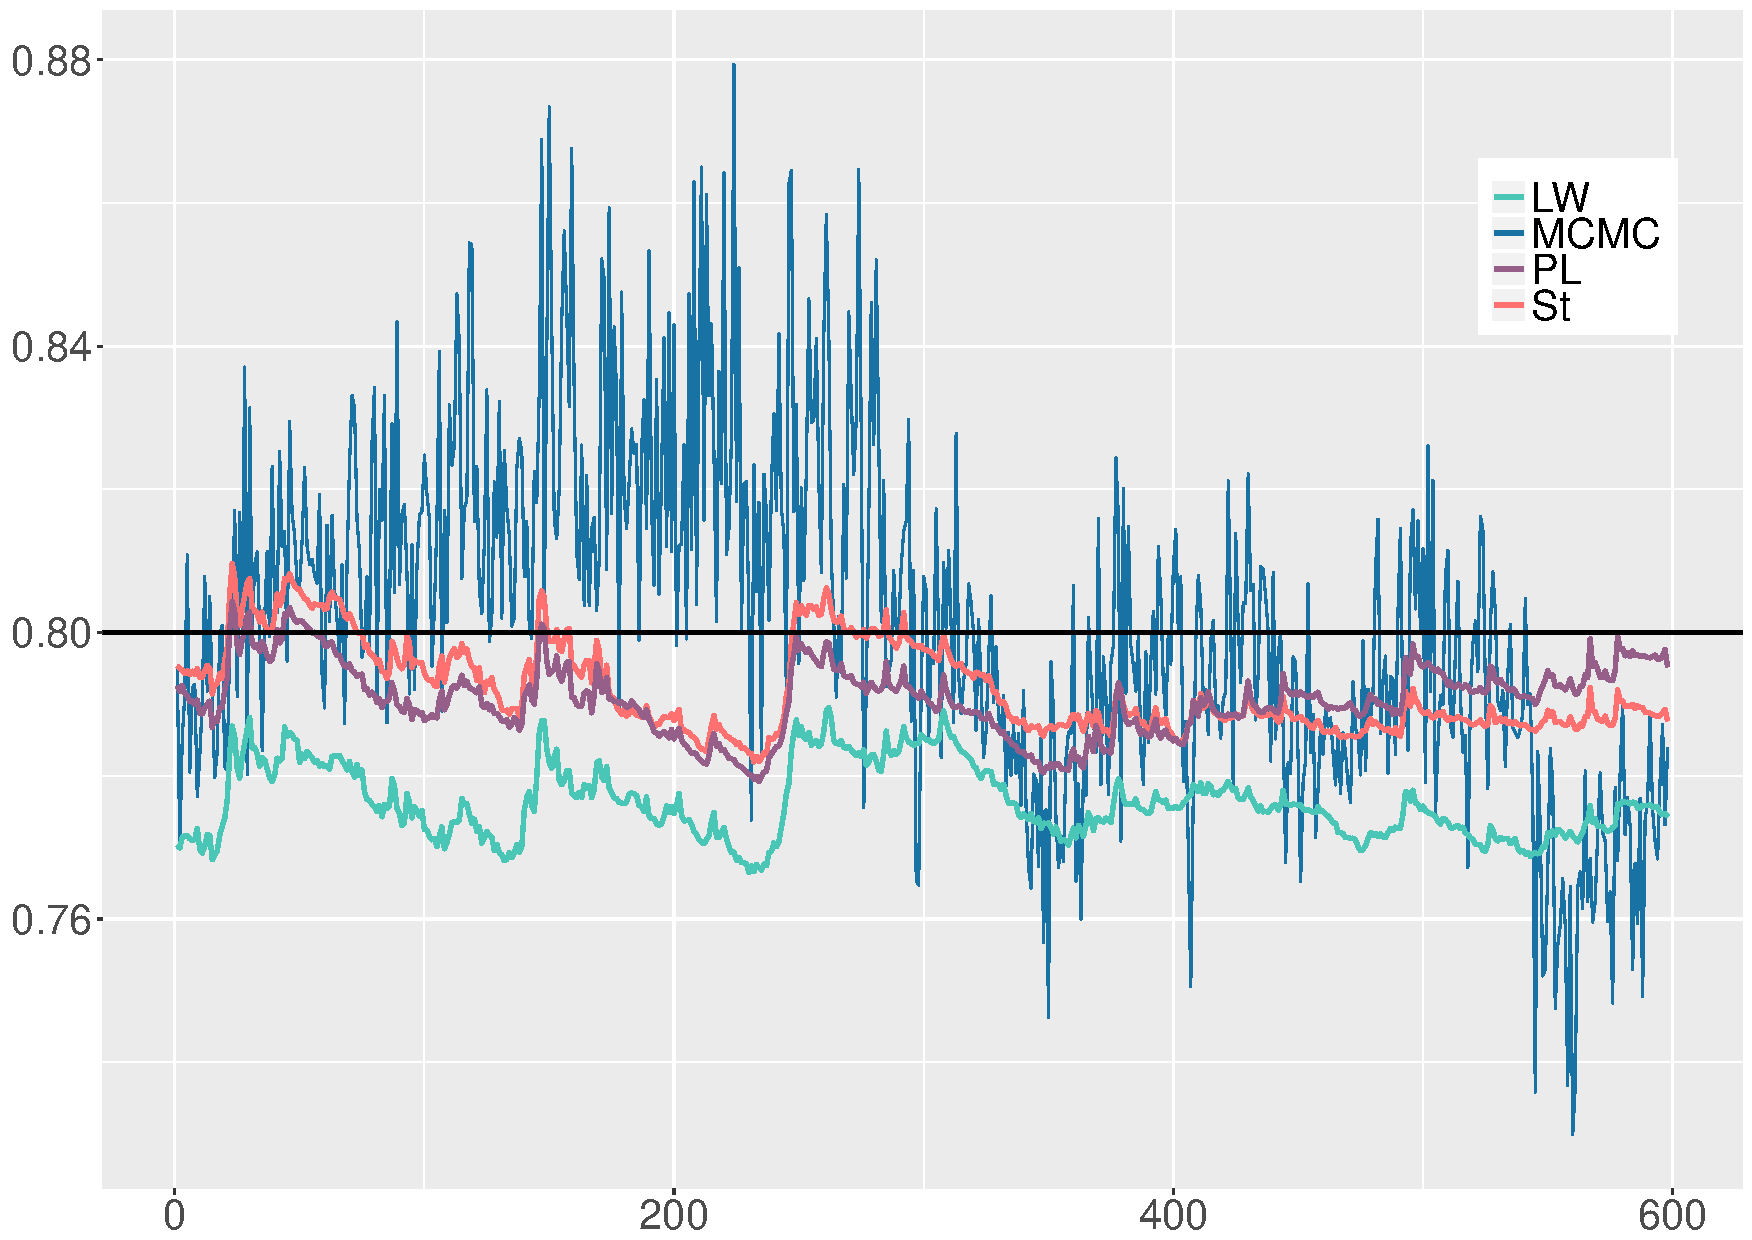
\includegraphics[width=0.45\textwidth]{Chapters/04Filtering/plot/ggFilterCompPhi2.pdf}
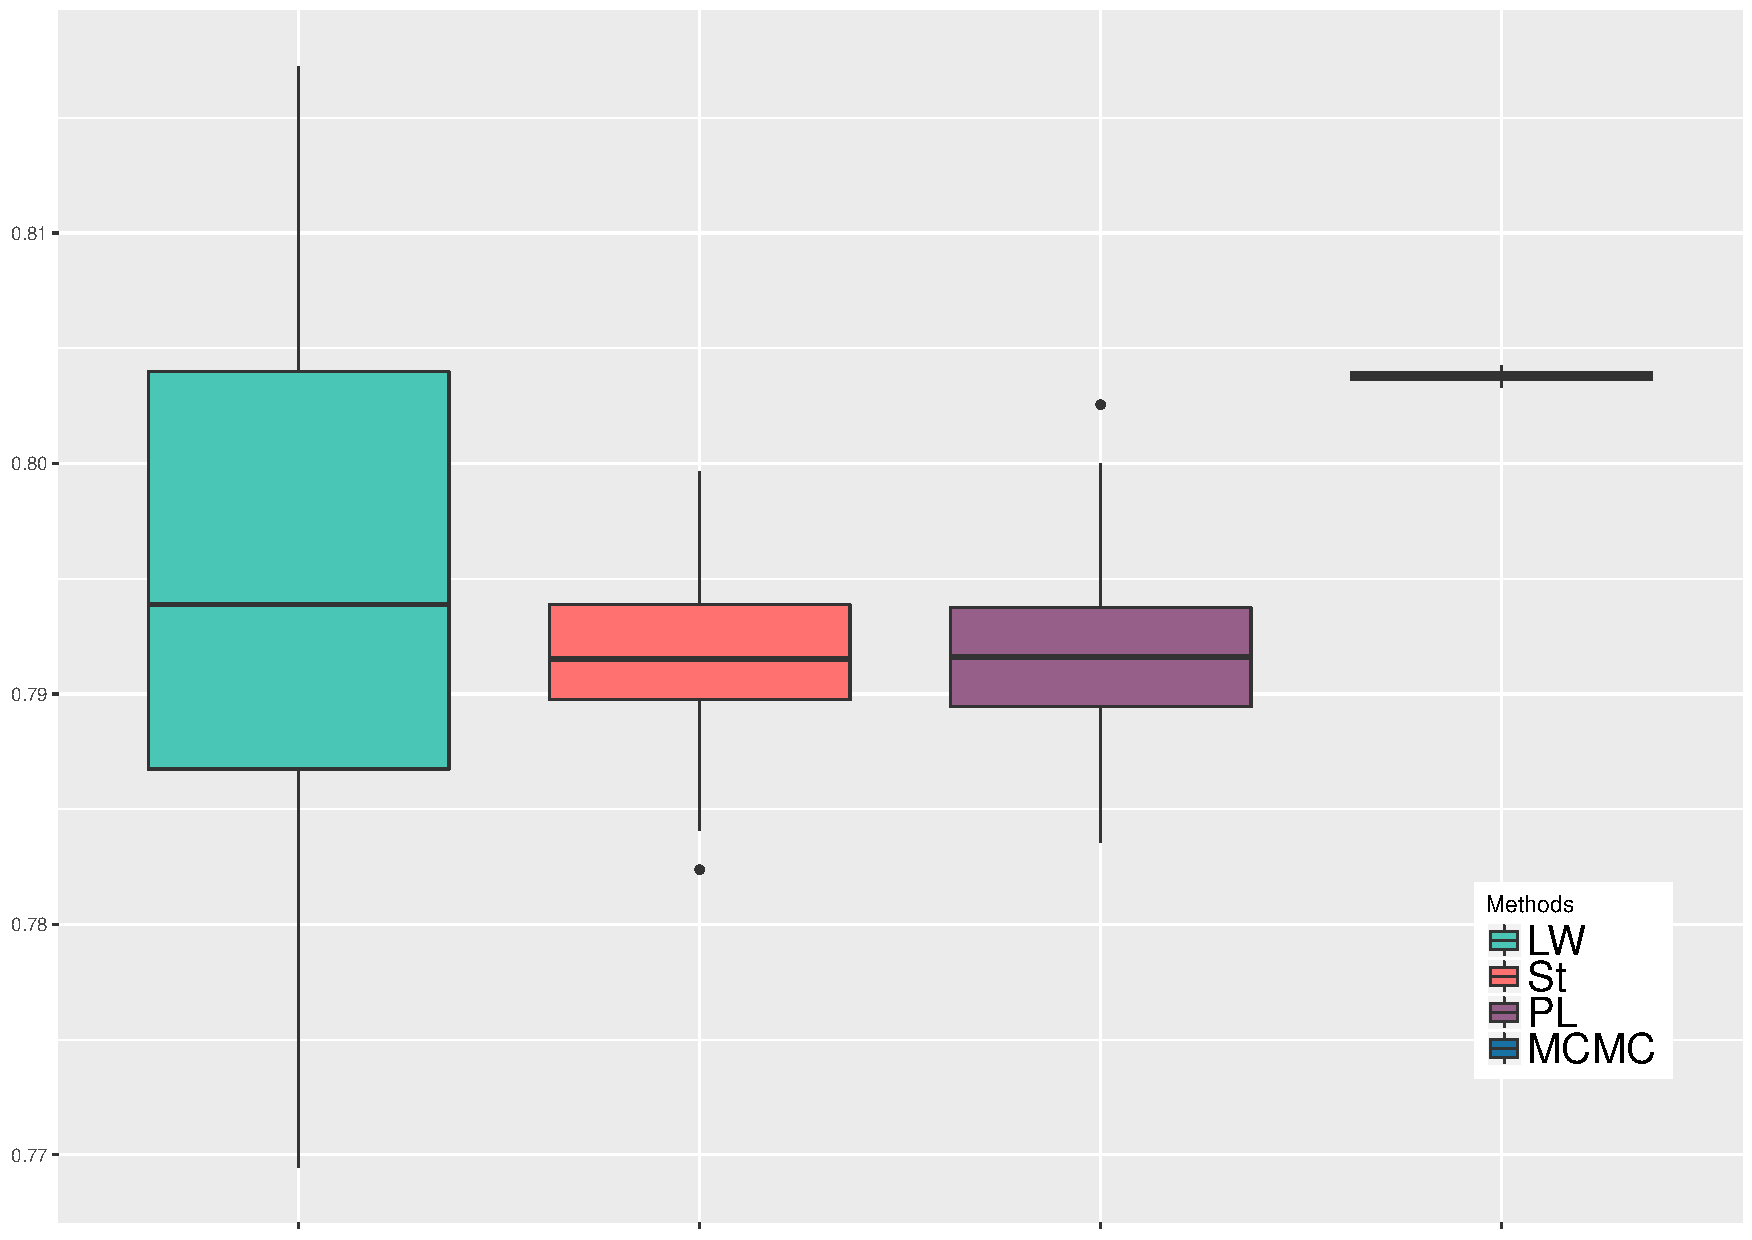
\includegraphics[width=0.45\textwidth]{Chapters/04Filtering/plot/ggBoxComp.pdf}
\caption{A comparison study using simulated time series data shows that LW, St and PL algorithms converge to the true $\phi$ at similar speed. The proposed MCMC algorithm has a higher variability. By repeatedly running for 50 times, the box-plot indicates that the proposed MCMC has a higher stability comparing with the other three algorithms. } \label{FilterRiewComparesion01}
\end{figure}



\begin{figure}[h]
\centering
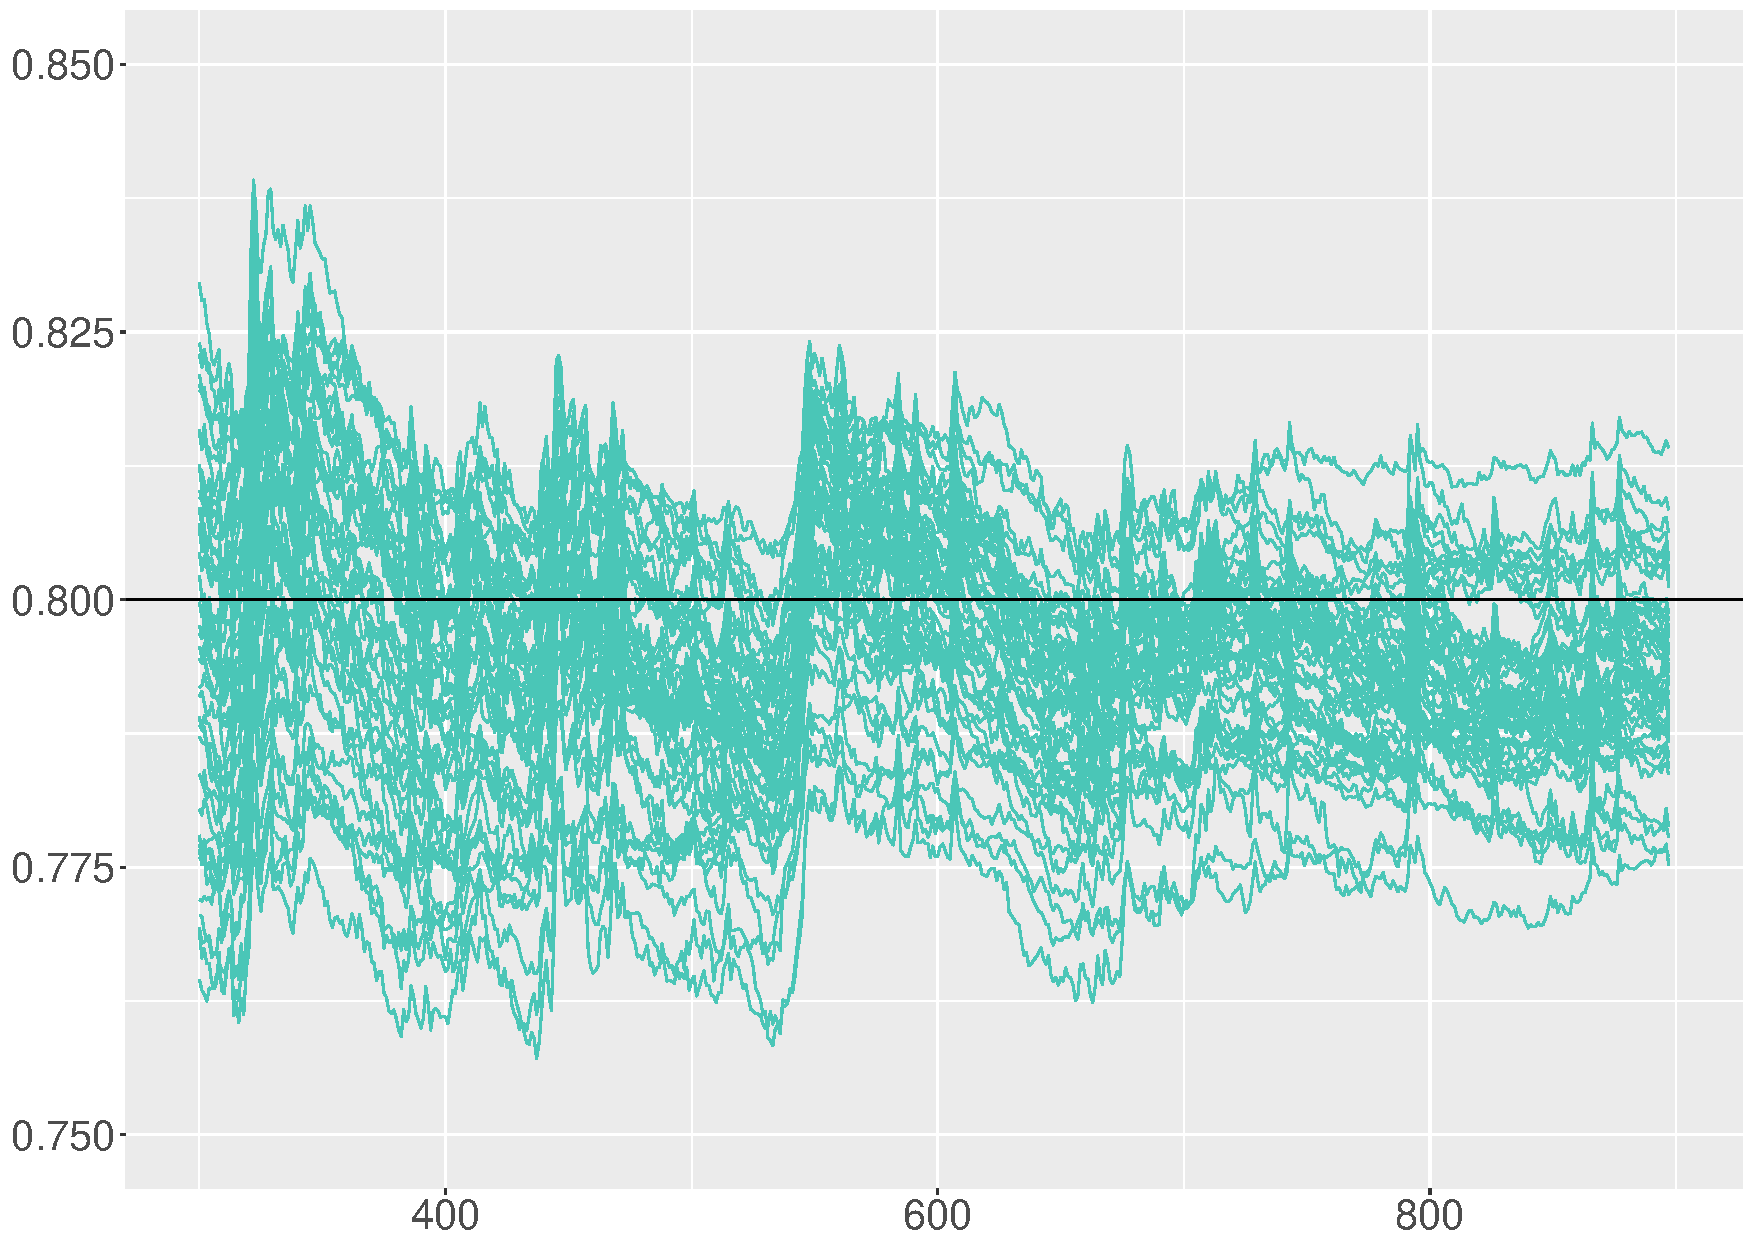
\includegraphics[width=0.45\textwidth]{Chapters/04Filtering/plot/LWchain100.pdf}
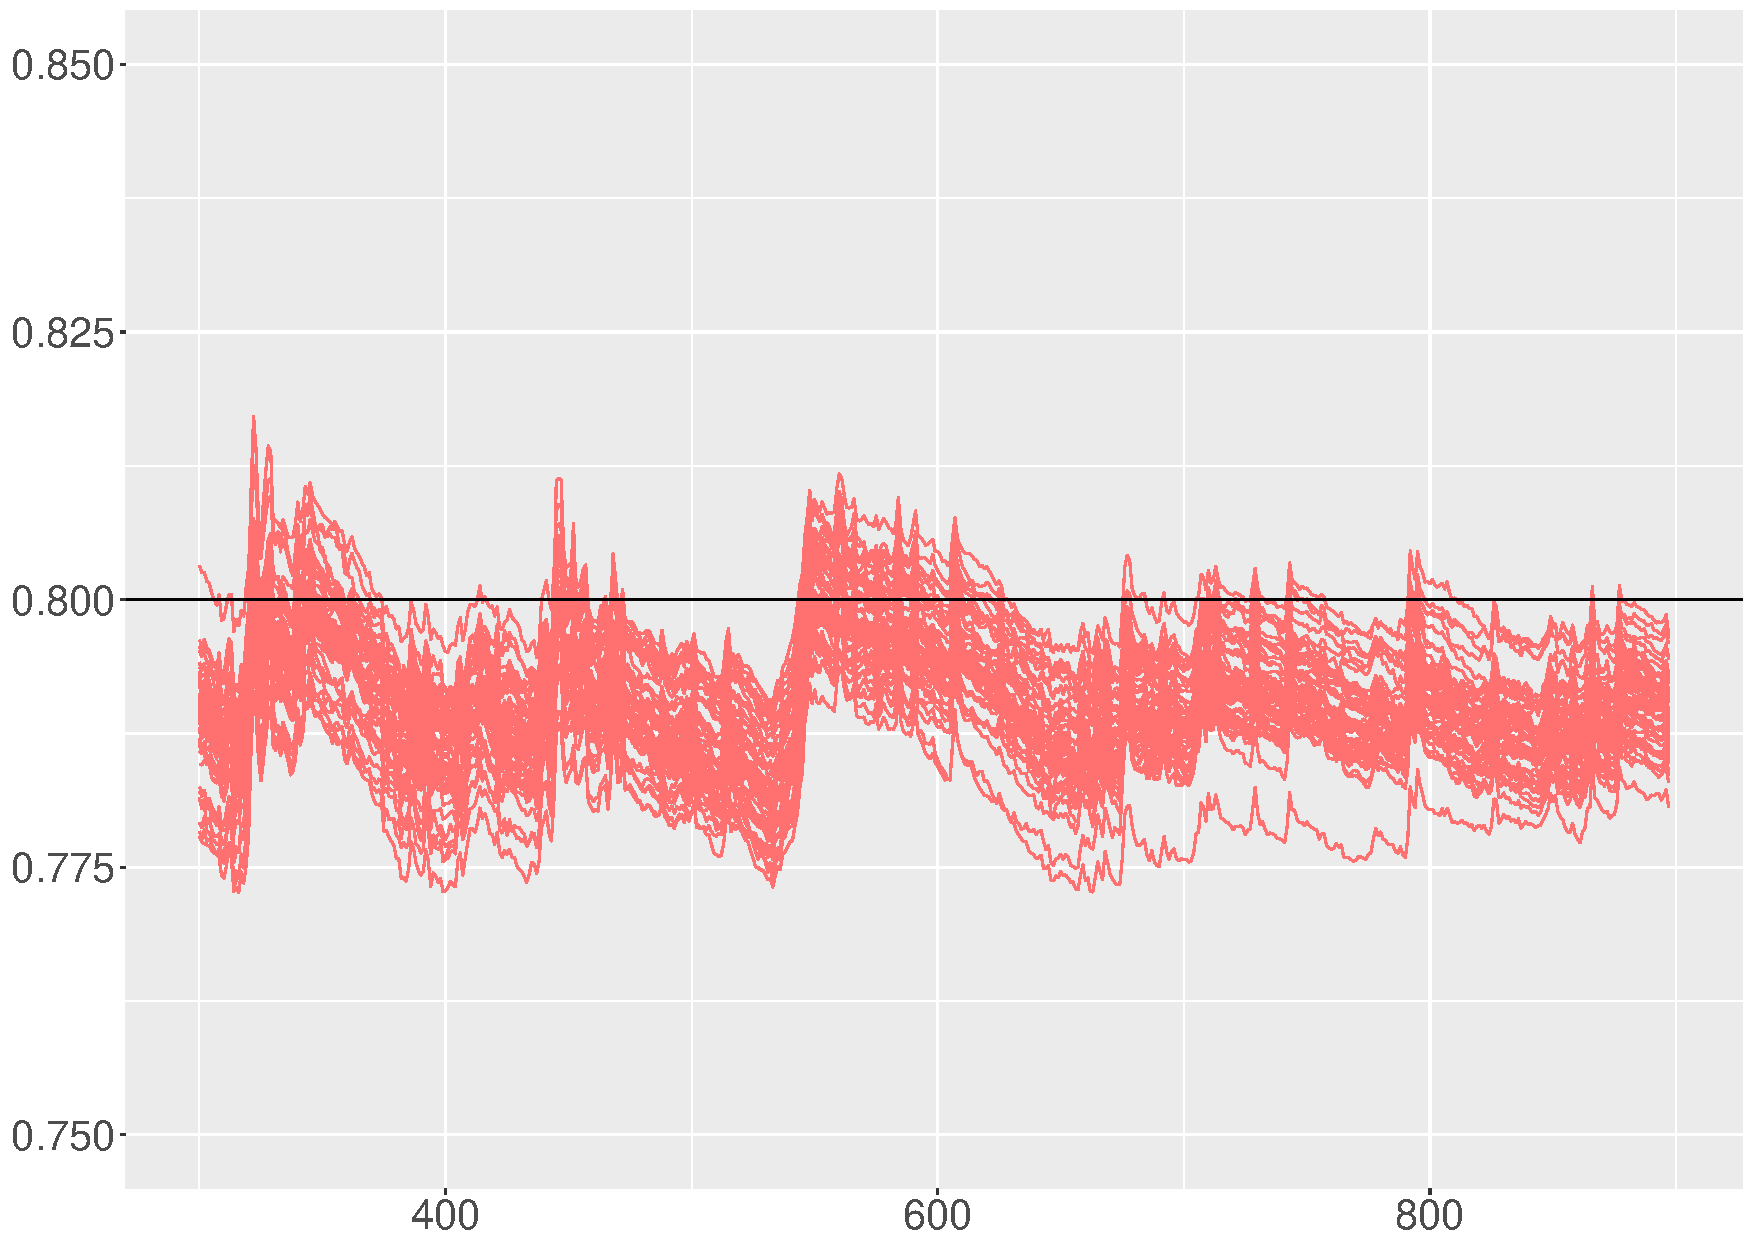
\includegraphics[width=0.45\textwidth]{Chapters/04Filtering/plot/STchain100.pdf}
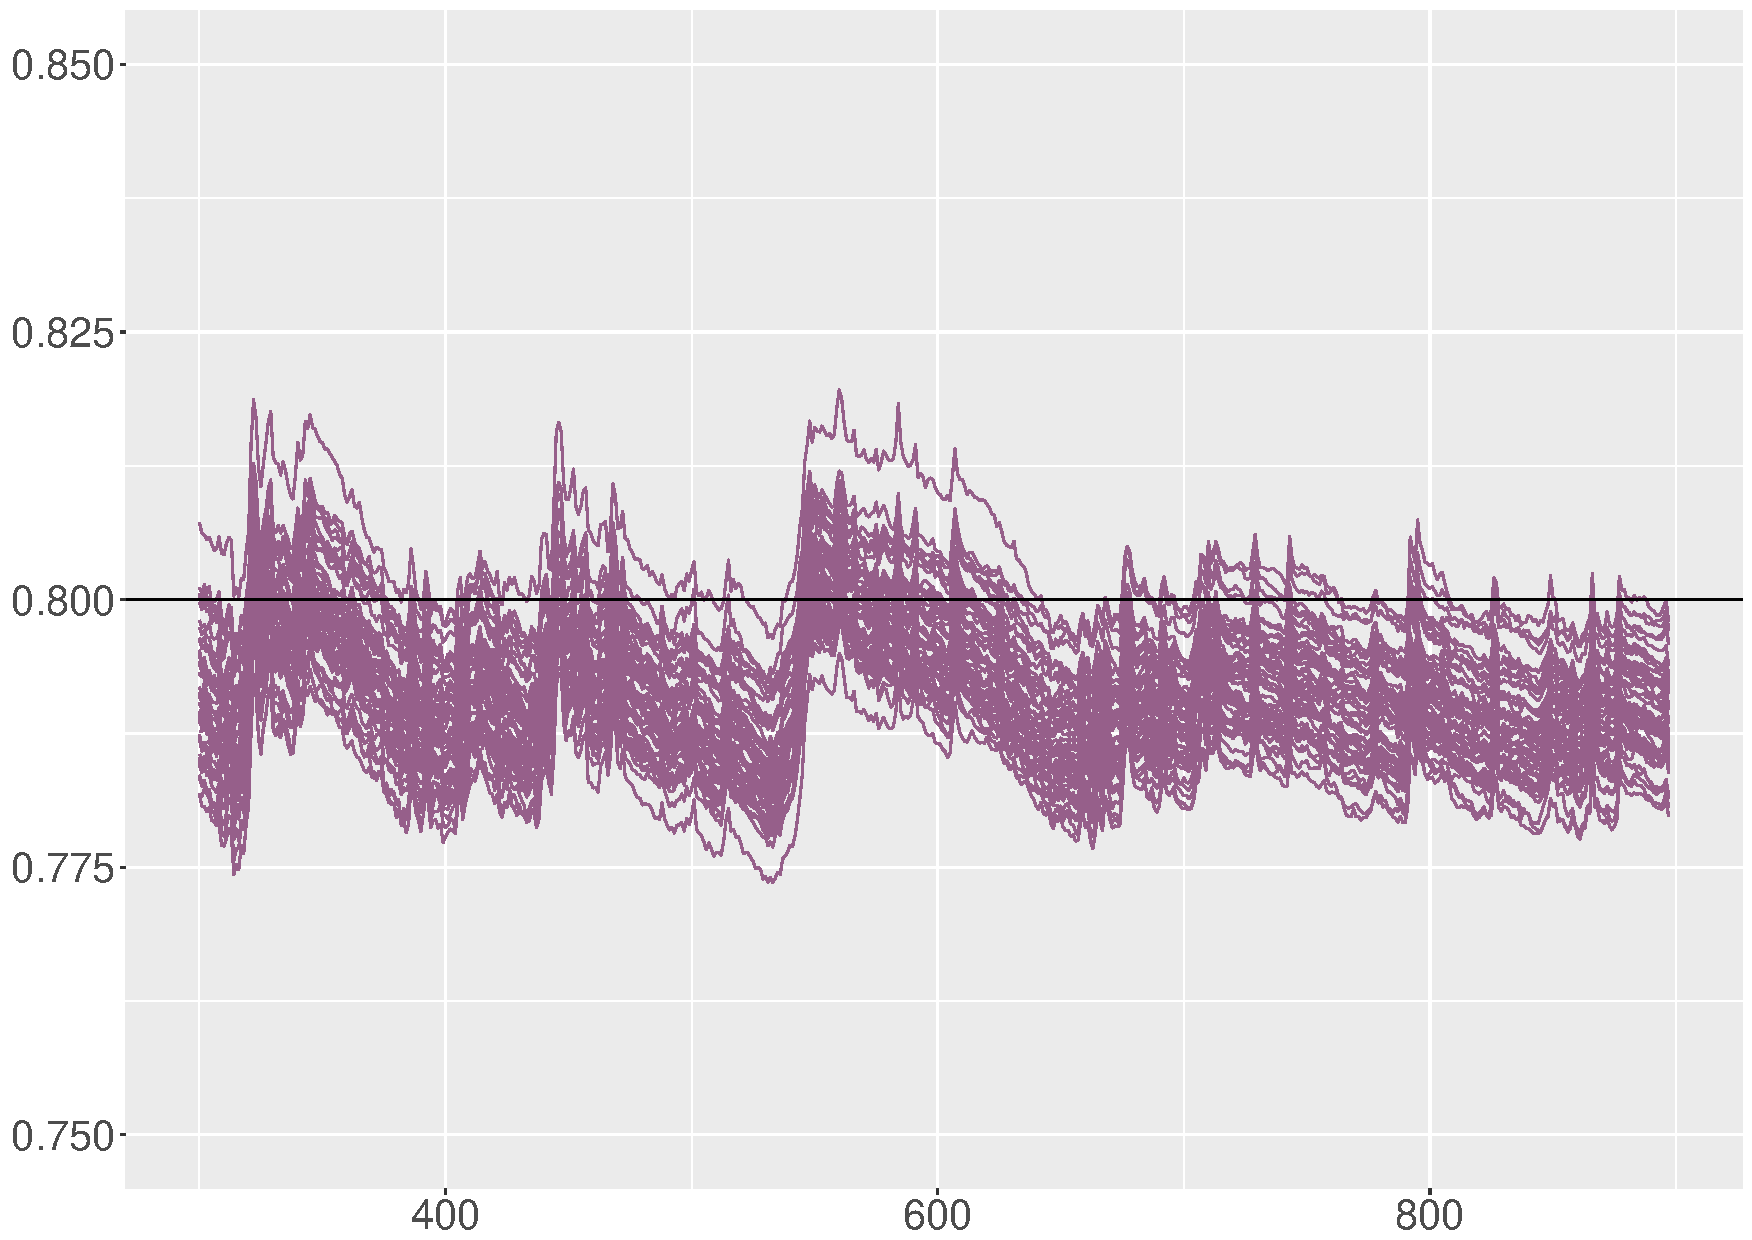
\includegraphics[width=0.45\textwidth]{Chapters/04Filtering/plot/PLchain100.pdf}
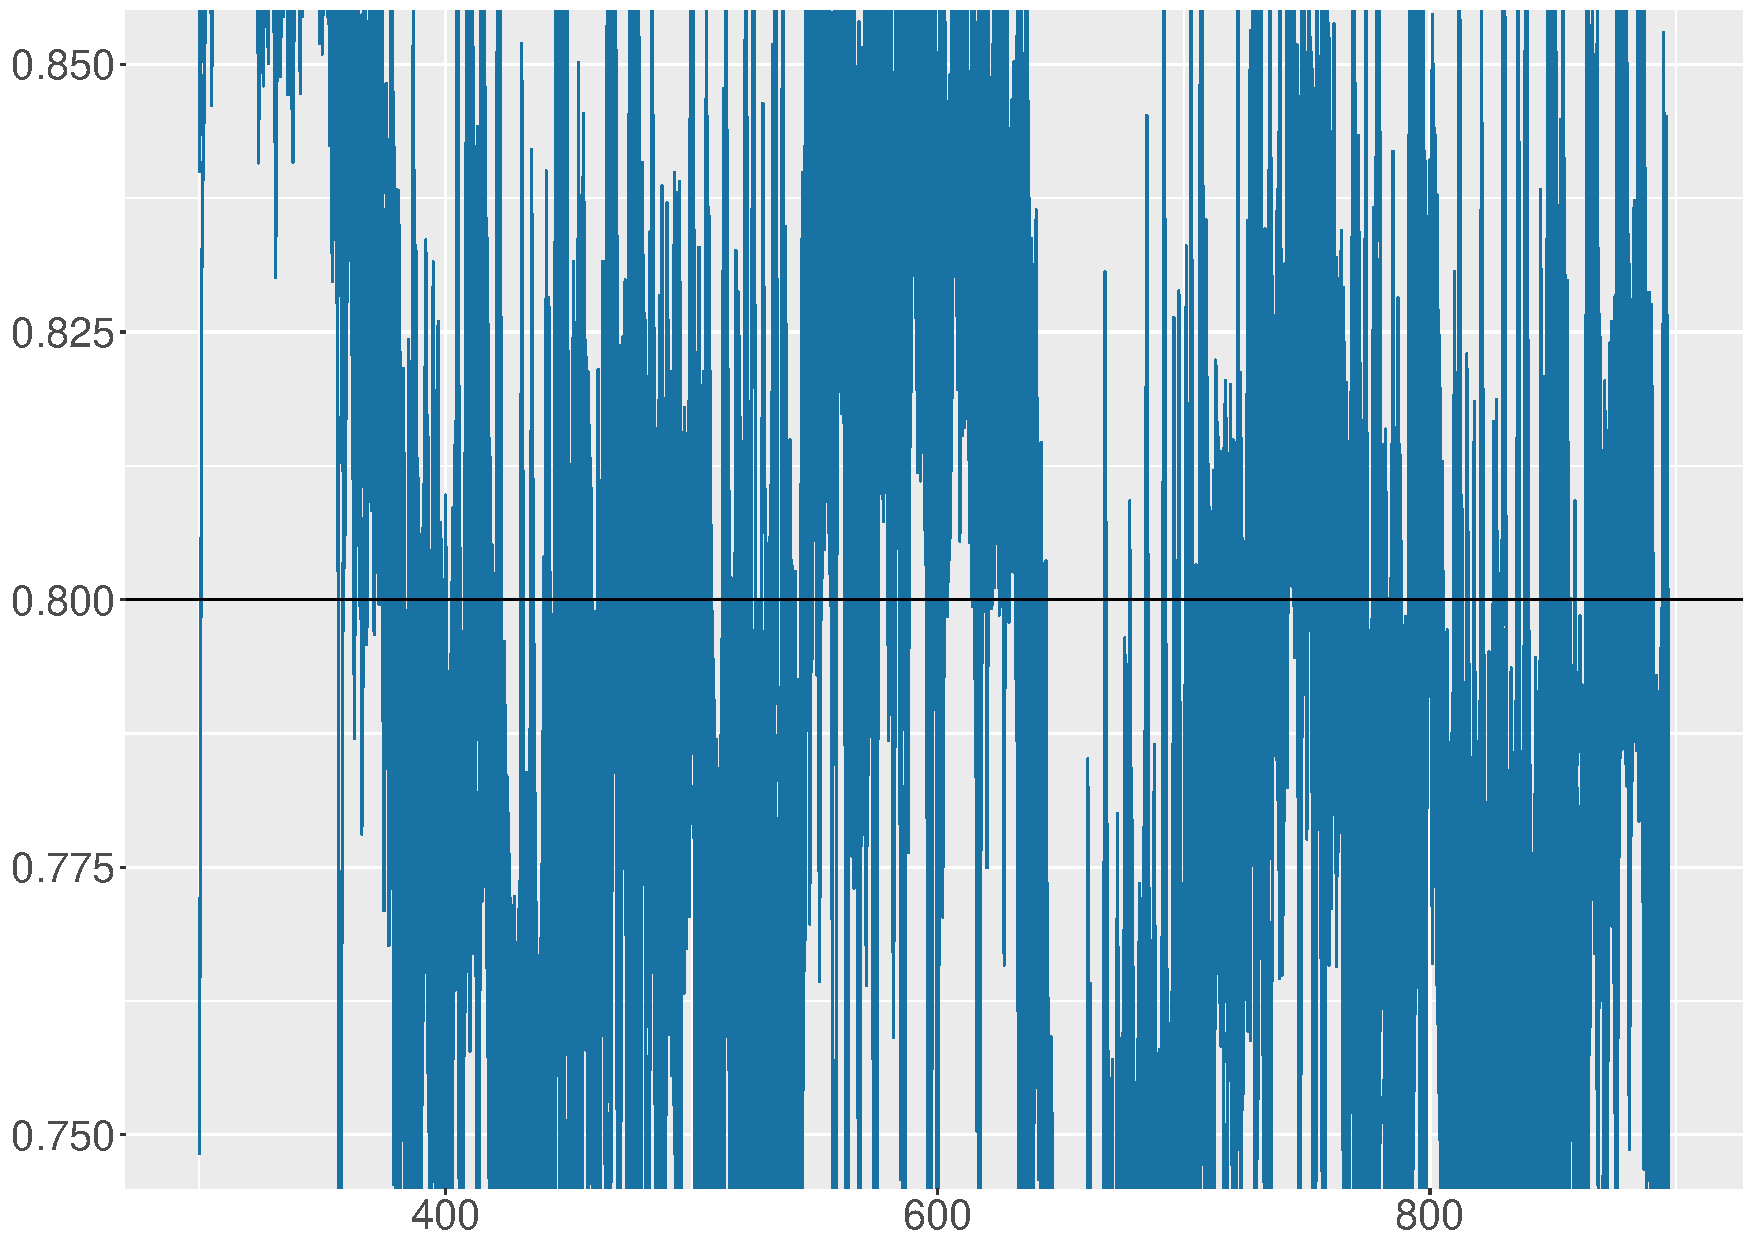
\includegraphics[width=0.45\textwidth]{Chapters/04Filtering/plot/MCMCchain100.pdf}
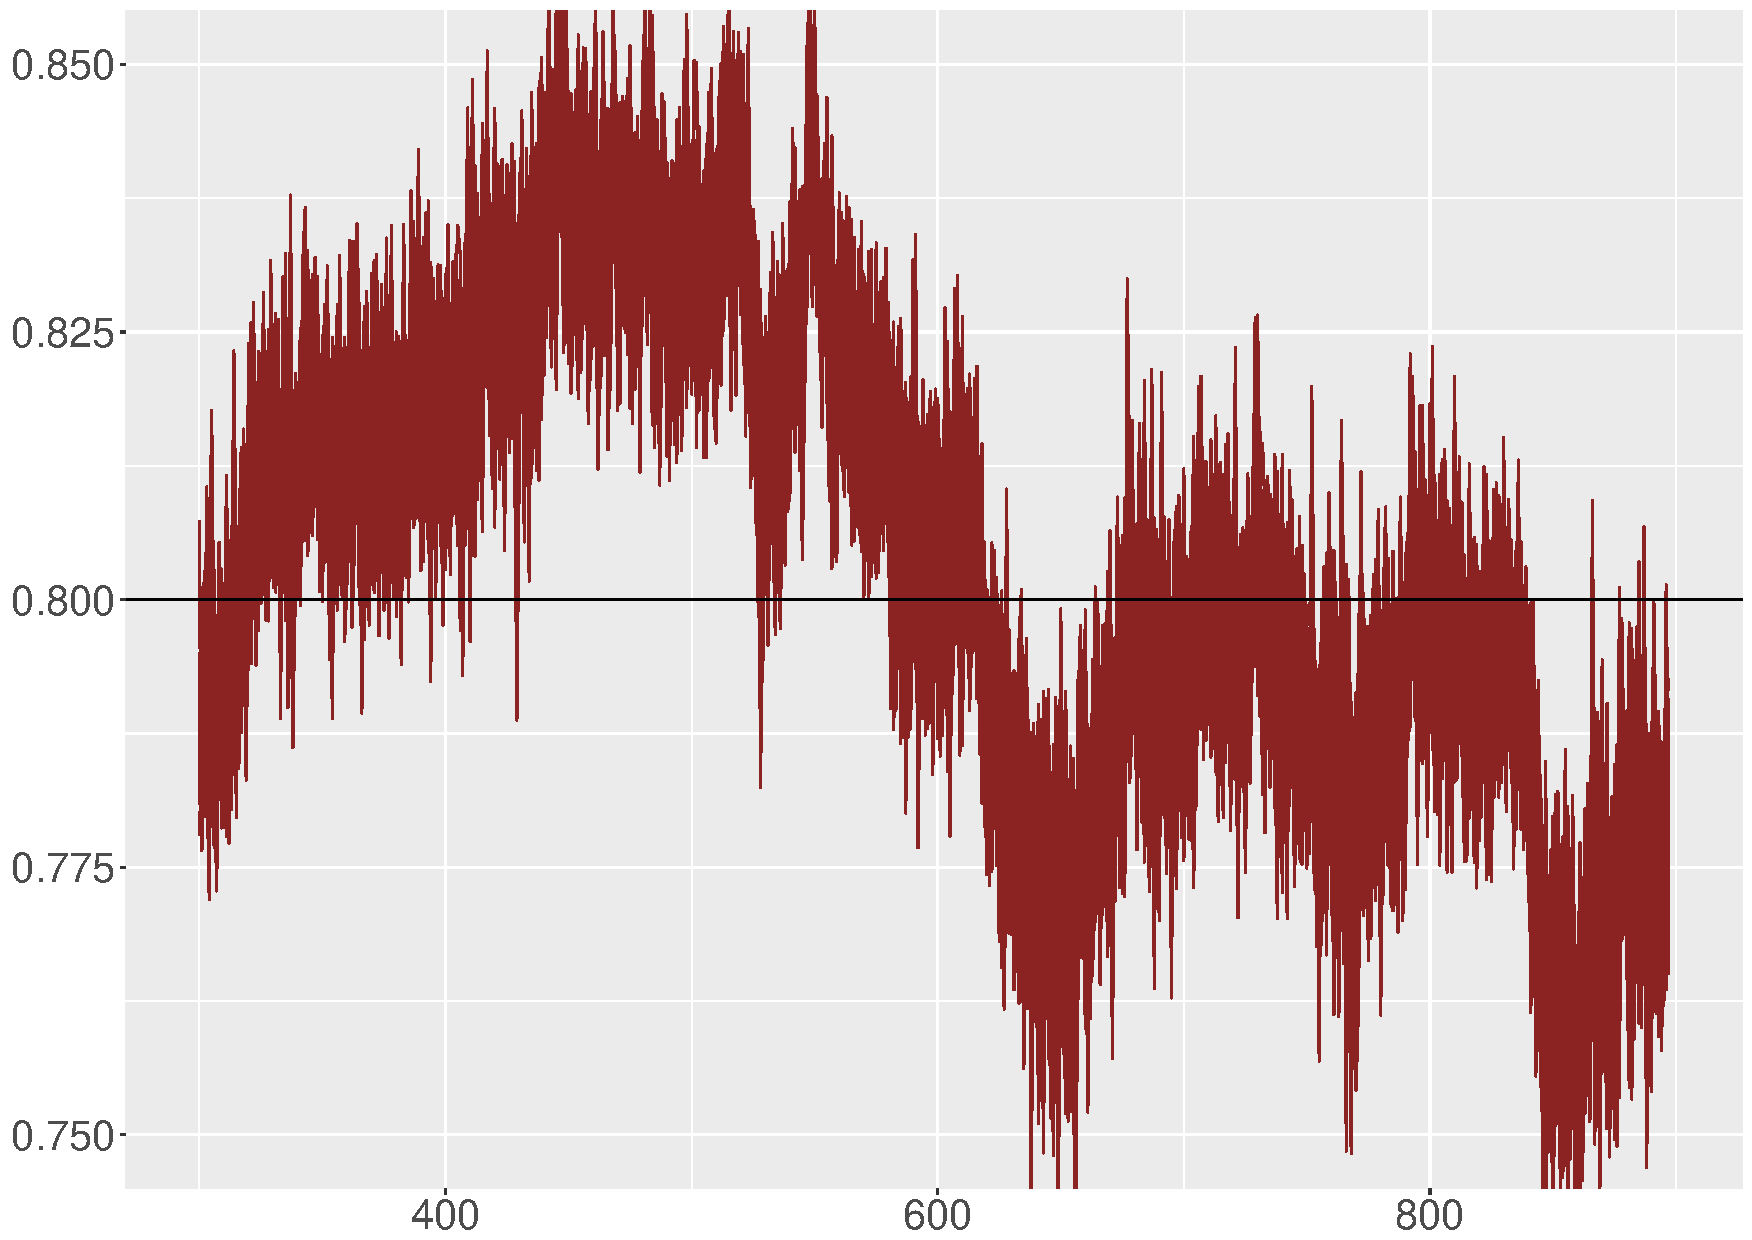
\includegraphics[width=0.45\textwidth]{Chapters/04Filtering/plot/MCMCchain300.pdf}
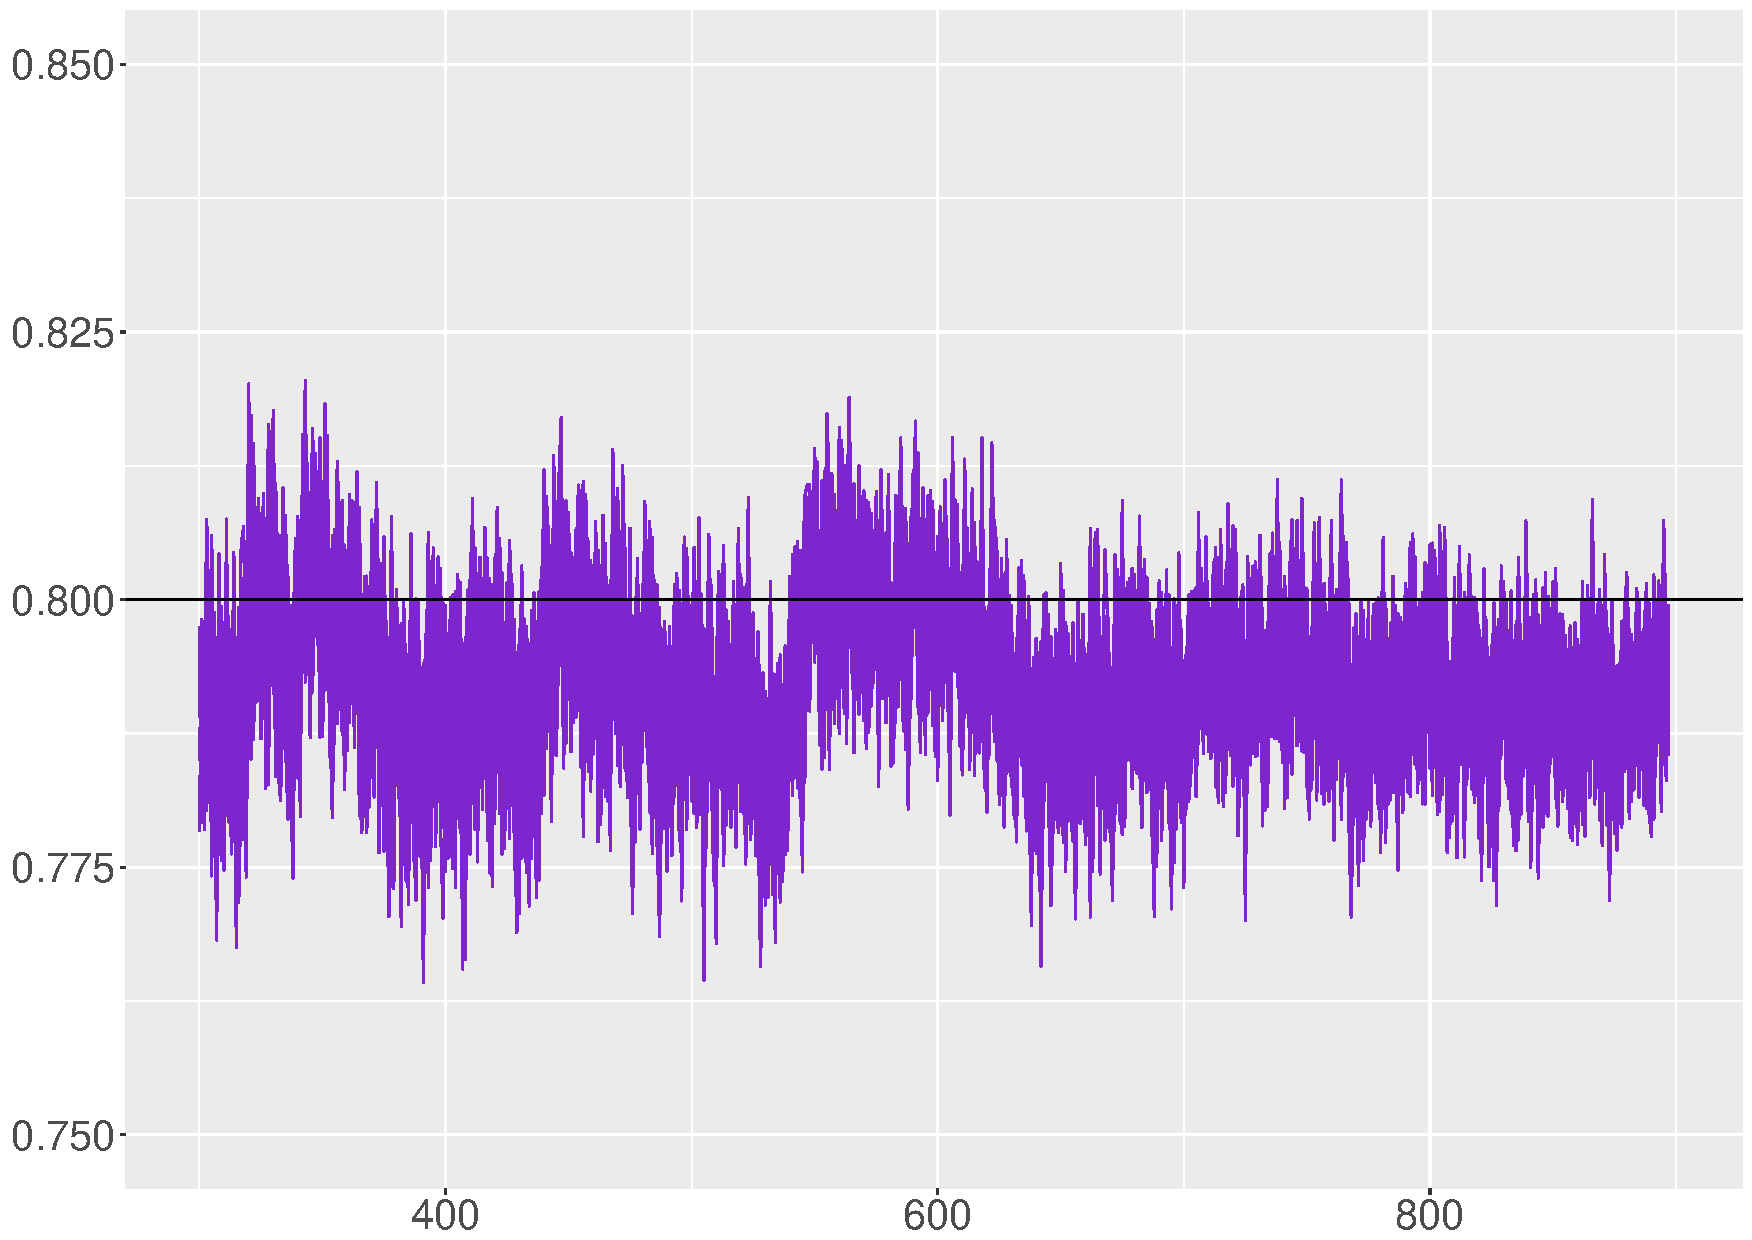
\includegraphics[width=0.45\textwidth]{Chapters/04Filtering/plot/MCMCchainVary.pdf}
\caption{Chain plots. Repeatedly running 50 times. Cutting off the first \textbf{300} data. LW, St, PL filters are using 5\,000 particles. MCMC is using 5\,000 samples. The lengths of sliding window MCMC-100 and MCMC-300 stay constant at \textbf{100} and \textbf{300}. The length of MCMC-vary expends along time $t$. }
\end{figure}

 
\begin{figure}[h]
\centering
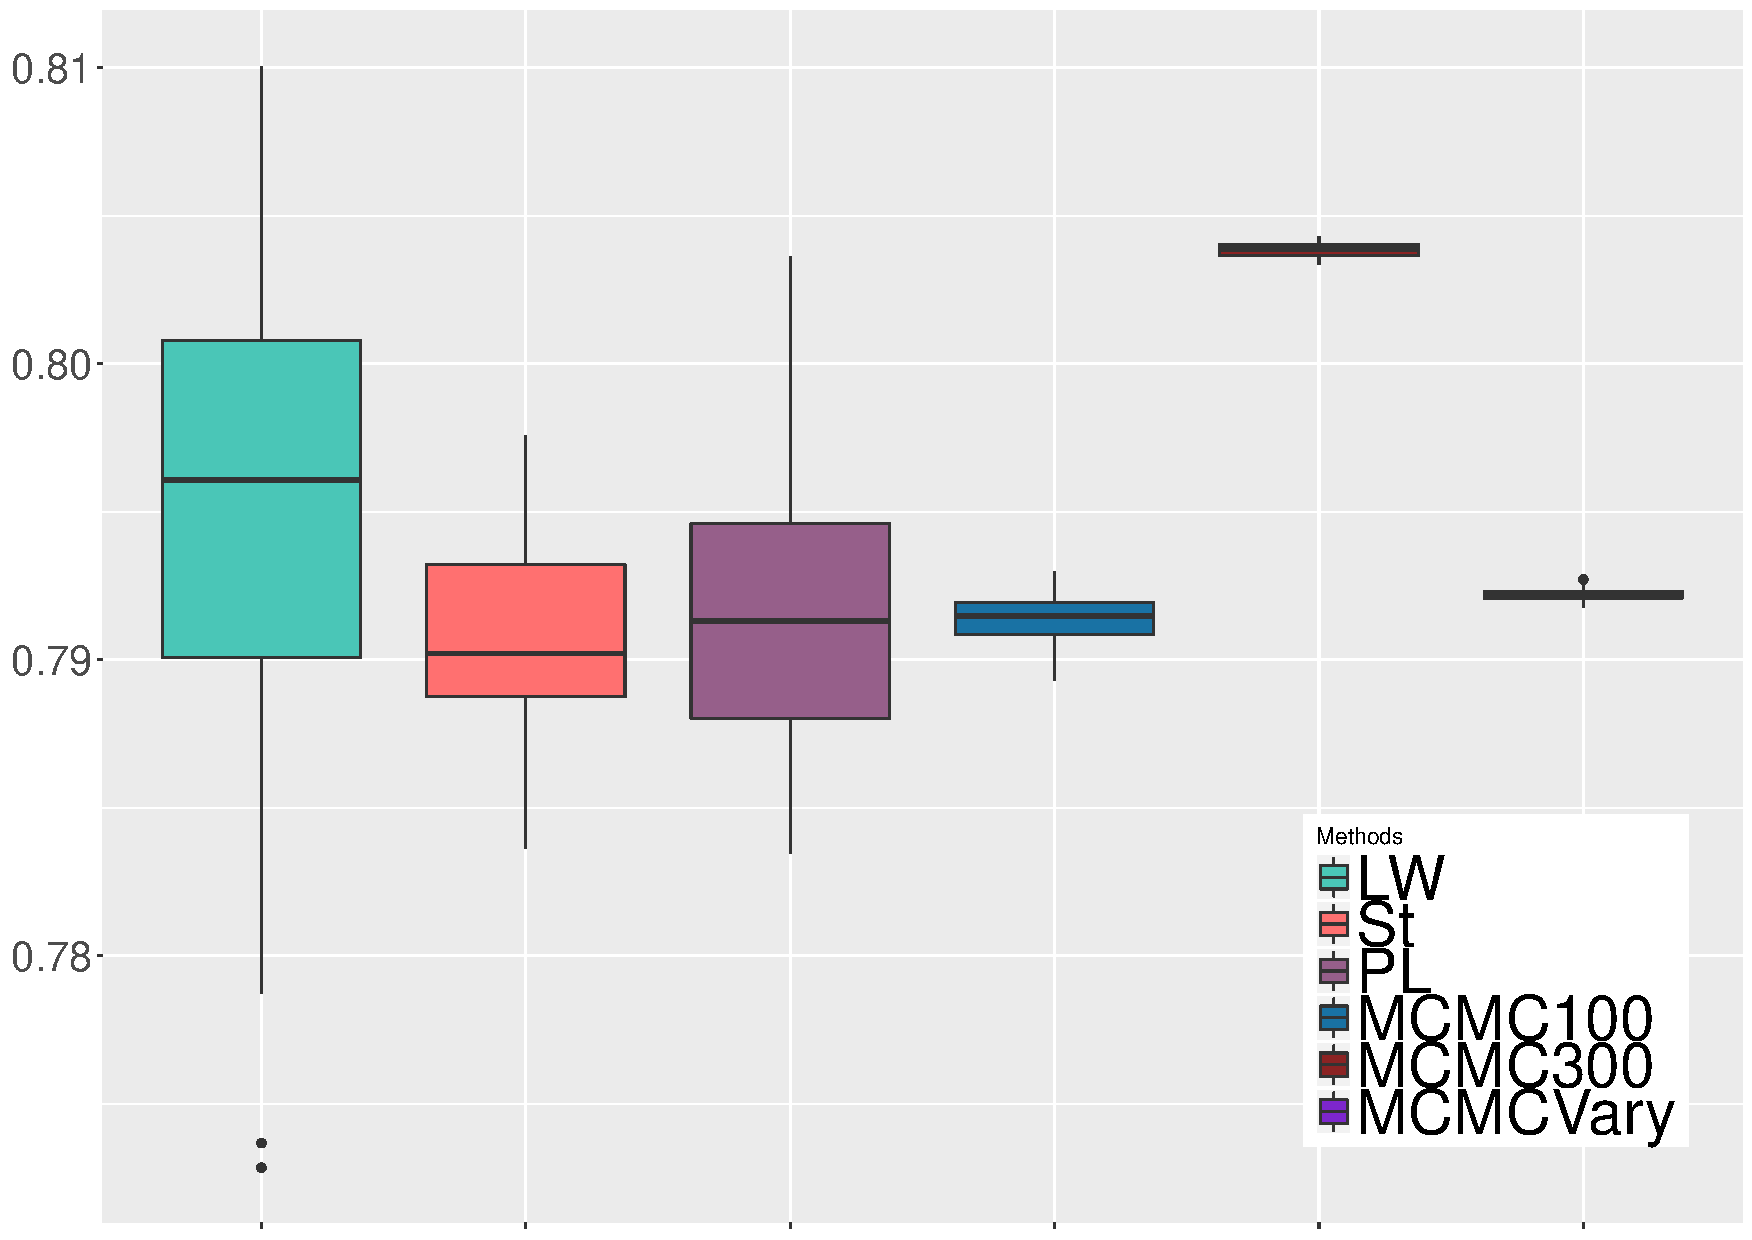
\includegraphics[width=0.95\textwidth]{Chapters/04Filtering/plot/CompMCMCboxplotALL.pdf}
\caption{Repeatedly running 50 times. Cutting off the first \textbf{300} data. LW, St, PL filters are using 5\,000 particles. MCMC is using 5\,000 samples. The length of sliding window MCMC stays constant \textbf{100} and \textbf{300}. The length of sliding window MCMC-vary is expanding along time $t$. For example, at $t=300$, the length is 300 ($y_{1:300}$); at $t=500$, the length is 500 ($y_{1:500}$). }
\begin{tabular}{|c|c|c|c|c|c|c|}
\hline
     & LW & St & PL  & MCMC-100 & MCMC-300 & MCMC-vary \\ \hline
Mean of $\hat{\phi}$ & 0.7947 &   0.7908   &  0.7918 & 0.7914 &  0.8038& 0.7922 \\ \hline
Se of $\hat{\phi}$ ($\times 10^{-4}$) &  13.1000  & 4.8793 & 6.2877 & 1.1388 & 0.3275 & 0.27506 \\ \hline
$\frac{1}{n}\sum_i(\hat{x}_i-x_i)^2$ & 0.5745 & 0.5739 & 0.5737 & 0.5875&  0.5741 &  0.5740 \\ \hline
\end{tabular}
\end{figure}



\begin{figure}[h]
\centering
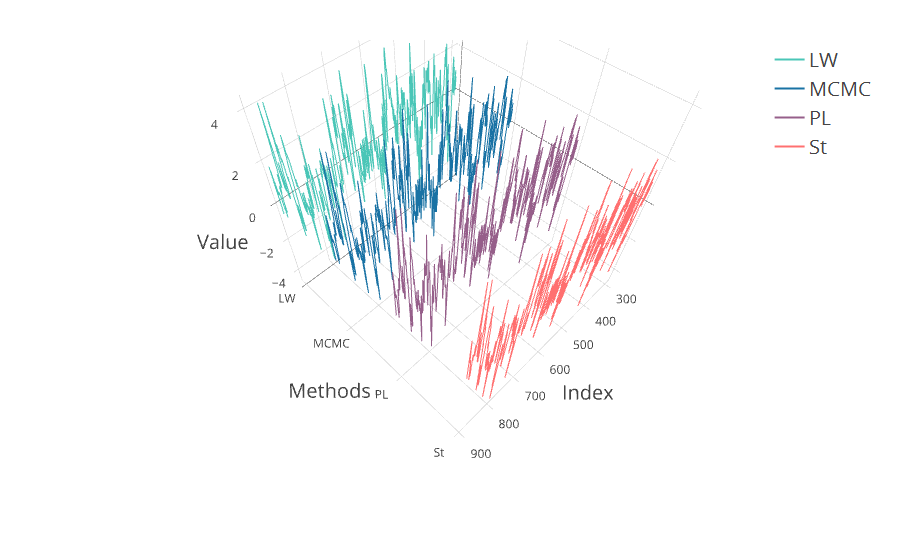
\includegraphics[width=\textwidth]{Chapters/04Filtering/plot/plotlyFilterCompX2.png}
\caption{The filtering for $x_{300:897}$ is very competitive. These four algorithms return very close estimations. } \label{FilterRiewComparesion02}
\end{figure}

\begin{table}[]
\centering
\caption{Comparison by repeatedly running 50 times with $N=5\,000$ particles for LW, St and PL and $M=5\,000$ samples for MCMC. }
\label{FilterRiewComparesionTable}
%\begin{tabular}{|c|c|c|c|}
%\hline
%     & Liu and West's & Storvik Filter & Particle Learning  \\ \hline
%MSE  &  0.5843 &  0.5842 &  0.5823     \\ \hline
%Time (seconds) &  213.27   &  296.70  & 272.62    \\ \hline
%Variance ($\times 10^{-4}$) &  7.3595   & 12.5294   & 11.7947    \\ \hline
%\end{tabular}
\begin{tabular}{|c|c|c|c|c|}
\hline
     & LW & St & PL  & MCMC\\ \hline
%Time (seconds) &  213.27   &  296.70  & 272.62   &  -- \\ \hline
%Median of $\hat{\phi}$ &  0.7944 (0.0070) &  0.7922(0.0098)   & 0.7907 (0.0116) &   0.8036 (0.0045) \\ \hline
%Variance of $\hat{\phi}$ ($\times 10^{-5}$) &  2.52  & 3.85  &  2.41 &   71.86  \\ \hline
%$\frac{1}{n}\sum_i(\hat{x}_i-x_i)^2$ &  0.5731 &  0.5750 &  0.5742  & 0.5744  \\ \hline
Median of $\hat{\phi}$ &  0.7944  &  0.7917   &  0.7919 & 0.8032 \\ \hline
SE of $\hat{\phi}$ ($\times 10^{-4}$) &  15.1861  &  4.6121 & 5.4162 &  $\mathbf{0.9182}$  \\ \hline
$\frac{1}{n}\sum_i(\hat{x}_i-x_i)^2$ &  0.5745 &  0.5740 &  0.5740 & 0.5744  \\ \hline
\end{tabular}
\end{table}


From figure (\ref{FilterRiewComparesion01}) it can be seen that the former three algorithms converge to the true parameter $\phi$ with similar speed along time $t$. LW filter has larger distance to the true parameter comparing with St and PL filters. The proposed MCMC algorithm has the biggest estimation variance. The estimations for $x_t$ from $t=300$ to $897$ are very close and hard to tell visually. From table (\ref{FilterRiewComparesionTable}), we can see that, by repeatedly running 50 times, the proposed MCMC algorithm is more stable in estimating parameter $\phi$ as it has the lowest standard error (SE) among all the algorithms. The MSE of all the algorithms on estimating $x$ are on the similar levels. 


\section{Conclusion}

In this chapter, we take a brief review on existing sequential state estimation and combined state and parameter estimation. Particle filter is an efficient method for state estimation, although the particles impoverishment is inevitable. Extended to this method, researchers are working on killing particles degeneracy and several accomplishments have been achieved. A new challenge is estimating the unknown parameters. In no doubt, for complex stochastic processes and dynamics, both  Bayesian and Frequentist methods are working well. 

In summary, most of research issues for filtering and parameter estimation focused on 
\begin{itemize}
\item Choices of resampling scheme to kill particles degeneracy, such as Liu and West's filter.
\item Exploration of an efficient sampling algorithm, such as Metropolis-Hastings sampler. 
\item Exploration of accurate estimation with low variances in higher dimensional space. 
\end{itemize}

Subject to pages and time, some algorithms are not included in the brief review. For more information and interests, readers can refer to unscented Kalman filter \cite{wan2000unscented} and its related algorithms for non-linear estimation, particle MCMC \cite{andrieu2010particle} for off-line Bayesian estimation and on-line gradient approach \cite{poyiadjis2005maximum} for parameter estimation. 



